\graphicspath{{Chapters/back_matter/Figures/}}
\appendix

\chapter{\tgp Data (Glycerol)} \label{app:GlycerolIGP}

\sisetup{
	round-mode          = places,
	round-precision     = 3,
}

\begin{table}[h!]
	\centering
	\caption{Glycerol \tgp Data}
	\label{table:IGPdataGlycerol}
	\pgfplotstabletypeset[
	multicolumn names,
	col sep=comma,
	display columns/0/.style={
		column name=Pressure,
		column type={S},
		string type
	},
	display columns/1/.style={
		column name=Temperature,
		column type={S},
		string type
	},
	display columns/2/.style={
		column name=Volume,
		column type={S},
		string type
	},
	every head row/.style={
		before row={\toprule},
		after row={
			\si{\giga\pascal} & \si{\kelvin} & \si{\cubic\centi\meter\per\gram}\\
			\midrule
		}
	},
	every last row/.style={after row=\bottomrule},
	]{Chapters/Back_matter/Figures/GlycerolTGPdata.csv}
\end{table}

\vspace{-0.5em}
{\small
	\noindent $^{*}$ Specific volumes corresponding to this pressure and above were obtained with moderate  to significant extrapolation of the Tait EOS beyond Bridgman's data.
	\par}

\begin{equation}
	\label{equ:IGPglycerol}
	T_{G}(P)=188.376\left ( 1+2.046\frac{P}{5.596} \right )^{\frac{1}{2.046}}
\end{equation}

\chapter{\tgp Data (Cumene)} \label{app:CumeneIGP}

\sisetup{
	round-mode          = places, % Rounds numbers
	round-precision     = 3, % to 2 places
}

\begin{table}[h!]
	\begin{center}
		\caption{Cumene \tgp Data}
		\label{table:IGPdata}
		\pgfplotstabletypeset[
		multicolumn names, % allows to have multicolumn names
		col sep=comma, % the separator in our .csv file
		display columns/0/.style={
			column name=Pressure, % name of first column
			column type={S},string type},  % use siunitx for formatting
		display columns/1/.style={
			column name=Temperature,
			column type={S},string type},
		display columns/2/.style={
			column name=Volume,
			column type={S},string type},
		every head row/.style={
			before row={\toprule}, % have a rule at top
			after row={
				\si{\GPa} & \si{\kelvin} & \si{\cubic\centi\meter\per\gram}\\ % the units seperated by &
				\midrule} % rule under units
		},
		every last row/.style={after row=\bottomrule}, % rule at bottom
		]{Chapters/Back_matter/Figures/CumeneTGPdata.csv} % filename/path to file
	\end{center}
\end{table}

\begin{equation}
\label{equ:IGPcumene}
T_{G}(P)=131.145\left ( 1+1.64181\frac{P}{1.21852} \right )^{\frac{1}{1.64181}}
\end{equation}

%cumene IGP data

\chapter{Equation of State (glycerol)} \label{app:GlycerolEOS}
To facilitate the conversion of glycerol pressure data ($\si{\giga\pascal}$) to molecular volume $\nicefrac{\si{\angstrom\cubed}}{molecule}$ the Tait equation of state, fit to Bridgman's glycerol data \cite{BridgmanGly}, was implemented.  It should be noted that Bridgman only obtained PVT data up to just under $1.2\;\si{\giga\pascal}$ yet Cook \etal extrapolates this equation of state up to $3\;\si{\giga\pascal}$ \cite{Cook2}. This work extrapolates this equation of state up to $6.68\;\si{\giga\pascal}$ to allow for the thermodynamic scaling assessment of \sect \ref{sec:GlycerolScaling}.  Clearly, experimental measurement of the glycerol equation of state at these elevated pressures is desperately needed yet remains absent within the literature.  However, despite dependence upon these extreme extrapolations, thermodynamic scaling of glycerol data implementing this equation of state yields self-consistent results as was demonstrated in \fig \ref{figure:GlycerolIGPScaling}. The isothermal Tait equation of state is given as follows:

\begin{equation} 
\frac{V}{V_0}=1-c\times ln\left(\frac{b+P}{b+P_0}\right),
\label{eqn:tait}
\end{equation}

\noindent where $P_0$ and $V_0$ are simply arbitrarily chosen reference values of pressure and volume, respectively, at a specific temperature.  For this work $P_0$ was set to atmospheric pressure and $V_0$ was found to be sufficiently well modeled as a linear function of temperature as follows:
\begin{equation}
V_0(T)=0.065T + 119.7,
\label{eqn:vo}
\end{equation} 
where temperature, T, is expected in ($\si{\degreeCelsius}$) and the resulting specific volume, $V_0$, is returned in units of ($\nicefrac{\si{\angstrom\cubed}}{molecule}$).  The density data for glycerol to which \eqn \ref{eqn:vo} was fit was taken from Cheng \nolinebreak\cite{Cheng}. The remaining fit parameters $c$ and $b$ may be trivially related to the bulk modulus $K_0$ and its pressure derivative $K_{0}^{'}$ via \eqn \ref{eqn:abtait}.   
\begin{equation} 
K_0=\frac{P_0}{c}+\frac{b}{c}\:\:\:\:\:\:
and\:\:\:\:\:\:
K_{0}^{'}=\frac{1}{c}-1-Log\left ( \frac{b}{b+P_0} \right )
\label{eqn:abtait}
\end{equation} 
The reported values of the bulk modulus, $K_0$, and its pressure derivative, $K_{0}^{'}$, calculated from five separate isothermal Tait equations of state by Cook \etal was fit to a third order polynomial model shown in \fig \ref{figure:GlycerolBulkMod}.  This enables accurate interpolation of $K_0$ and $K_{0}^{'}$ at any arbitrary temperature within this range.
\begin{figure}[H]
\centering
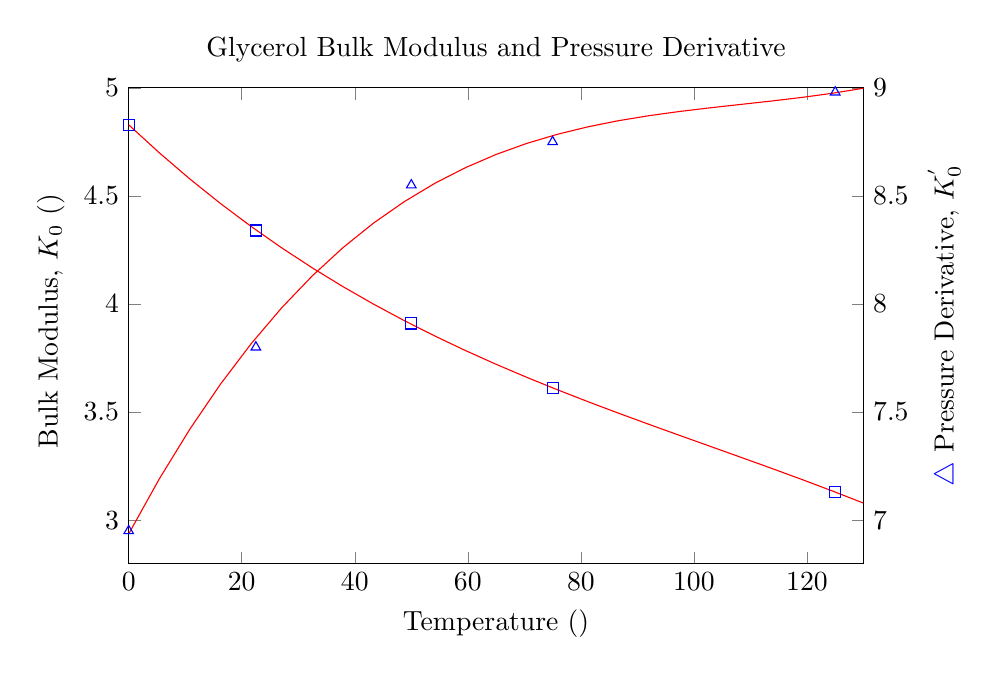
\begin{tikzpicture} 
\begin{axis}[
title={Glycerol Bulk Modulus and Pressure Derivative},
ylabel={$\color{blue}\square$ Bulk Modulus, $K_0$ ($\si{\giga\pascal}$)},
xlabel={Temperature ($\si{\degreeCelsius}$)},
ymin=2.8, ymax=5,
xmin=0, xmax=130,
%xtick={0,.002,.004,.006,.008,.01},
ytick={3,3.5,4,4.5,5},
width=0.9\textwidth,
height=3in
]

	\addplot+[only marks, mark=square]
	coordinates { 
		(0,4.83)
		(22.5,4.34)
		(50,3.91)
		(75,3.61)
		(125,3.13)};
	
	\addplot expression[domain=0:130,mark=none,red]{
	-0.00000048585*x^3+0.00014985*x^2-.024734*x+4.8291};
	
\end{axis}

\begin{axis}[
xmin=0,xmax=130,
ymin=6.8,ymax=9,
ytick={7,7.5,8,8.5,9},
axis y line*=right,
axis x line=none,
ylabel style = {align=center},
ylabel={$\color{blue}\triangle$ Pressure Derivative, $K_{0}^{'}$},
width=.9\textwidth,
height=3in
]

	\addplot+[only marks, mark=triangle]
	coordinates { 
		(0,6.95)
		(22.5,7.8)
		(50,8.55)
		(75,8.75)
		(125,8.98)};
	
	\addplot expression[domain=0:130,mark=none,red]{
	0.0000013142*x^3-0.00042776*x^2+.049260*x+6.9364};

\end{axis}

\end{tikzpicture}
\caption{The glycerol bulk modulus, $K_0$, and its pressure derivative, $K_{0}^{'}$, as extracted from reference \cite{Cook2} are provided above.  Each are fit to a third order polynomial to allow for interpolation to arbitrary temperatures within the range of $0\;\si{\degreeCelsius}$ to $130\;\si{\degreeCelsius}$. }
\label{figure:GlycerolBulkMod}
\end{figure}
From the interpolated values of the glycerol bulk modulus and its first pressure derivative, the c and b constants of the Tait model provided in \eqn \ref{eqn:tait} can be obtained via the simultaneous solution of \eqn \ref{eqn:abtait}.

\chapter{Equation of State (cumene)} \label{app:CumeneEOS}
All conversions from pressure to density or specific volume for cumene in this work were obtained via the modified Tait equation of state developed by Tim Ransom as shown in equation \ref{eqn:CumeneTait} below \cite{RansomPRL}. The density as a function of temperature at atmospheric pressure, $\rho_{0}(T)$, was provided by Cibulka \cite{Cibulka}.

\begin{equation}
	\begin{split}
		\:&\rho(T,P)=\frac{\rho_{0}(T)}{1-C(T)ln\left ( \frac{B(T)+P}{B(T)+0.0001\:\: \si{\giga\pascal}} \right )}\\\\
		&\text{for vectors}:\\
		&B(T)=\sum_{j=0}^{4}b_{j}\left [  \frac{T-T_{0}}{100}\right ]^j\:\:\:\:\:\:\:\:\text{and}\:\:\:\:\:\:\:\:C(T)=\sum_{j=0}^{1}c_{j}\left [  \frac{T-T_{0}}{100}\right ]^j\\
		& \text{where}\:\:\:\:\:\:\:\:T_{0}= 298.15\:\:\si{\kelvin}\:\:\:\:\:\:\:\:\text{and}:\\
		&\vec{b}=\begin{pmatrix}
			0.11110\:\: \si{\giga\pascal}\\ 
			-0.080954\: \si{\giga\pascal\per\kelvin}\\ 
			0.0226\:\: \si{\giga\pascal\per\kelvin\squared}\\ 
			-0.0034\:\: \si{\giga\pascal\per\kelvin\cubed}\\ 
			0.00028\:\: \si{\giga\pascal\per\kelvin\tothe{4}}\\
		\end{pmatrix} \:\:\:\:\:\:\:\:
		\vec{c}=\begin{pmatrix}
			0.093736 \\ 
			-0.0040032\: \si{\per\kelvin}\\ 
		\end{pmatrix}
	\end{split}
	\label{eqn:CumeneTait}
\end{equation}

\sisetup{
	round-mode          = places, % Rounds numbers
	round-precision     = 3, % to 2 places
}

\chapter{Cumene Data} \label{app:DPCSdata}
\begin{longtable}{ccccc}
	\caption{Cumene $\alpha$\--relaxation data}\label{table:DPCSdata}\\
	\toprule
	Pressure & Temperature & Volume & $Log_{10}(\tau_{cd})$ & Surface Error\textsuperscript{*} \\
	\si{\GPa} & \si{\kelvin} & \si{\cubic\centi\meter\per\gram} & \si{\pico\second} & \% \\
	\midrule
	\endfirsthead
	
	\toprule
	Pressure & Temperature & Volume & $Log_{10}(\tau_{cd})$ & Surface Error \\
	\si{\GPa} & \si{\kelvin} & \si{\cubic\centi\meter\per\gram} & \si{\pico\second} & \% \\
	\midrule
	\endhead
	
	\bottomrule
	\endfoot
	
	% -------- DPCS --------
	\csvreader[
	head to column names,
	late after line=\\
	]{Chapters/Back_matter/Figures/DPCSdata.csv}{}%
	{
		\num[round-mode=places,round-precision=2]{\csvcoli} &
		\num[round-mode=places,round-precision=2]{\csvcolii} &
		\num[round-mode=places,round-precision=3]{\csvcoliii} &
		\num[round-mode=places,round-precision=2]{\csvcoliv} &
		\num[round-mode=places,round-precision=2]{\Error}\%
	}
	
	% -------- DBLS --------
	\csvreader[
	head to column names,
	late after line=\\
	]{Chapters/Back_matter/Figures/DBLSdata.csv}{}%
	{
		\num[round-mode=places,round-precision=2]{\csvcoli} &
		\num[round-mode=places,round-precision=2]{\csvcolii} &
		\num[round-mode=places,round-precision=3]{\csvcoliii} &
		\num[round-mode=places,round-precision=2]{\csvcoliv} &
		\num[round-mode=places,round-precision=2]{\Error}\%\textsuperscript{$\dagger$}
	}
	
	% -------- Hansen OOOM-BOPP--------
	\csvreader[
	head to column names,
	late after line=\\
	]{Chapters/Back_matter/Figures/Hansendata.csv}{}%
	{
		\num[round-mode=places,round-precision=2]{\csvcoli} &
		\num[round-mode=places,round-precision=2]{\csvcolii} &
		\num[round-mode=places,round-precision=3]{\csvcoliii} &
		\num[round-mode=places,round-precision=2]{\csvcoliv} &
		\num[round-mode=places,round-precision=2]{\Error}\%\textsuperscript{$\ddagger$}
	}
	
	% -------- TGP / Isochrone --------
	\csvreader[
	head to column names,
	late after line=\\
	]{Chapters/Back_matter/Figures/TGPdata.csv}{}%
	{
		\num[round-mode=places,round-precision=2]{\csvcoli} &
		\num[round-mode=places,round-precision=2]{\csvcolii} &
		\num[round-mode=places,round-precision=3]{\csvcoliii} &
		\num[round-mode=places,round-precision=2]{\csvcoliv} &
		\num[round-mode=places,round-precision=2]{\Error}\%\textsuperscript{$\S$}
	}
	
\end{longtable}

\noindent\textsuperscript{*}Surface error is defined as the percent difference in $\log_{10}(\tau)$ between the measured relaxation times and the Andersson--Andersson zero-mobility constrained surface model shown in \fig~\ref{fig:SurfaceZeroMobilityFit}.

\noindent\textsuperscript{$\dagger$}Data correspond to Brillouin (DBLS) measurements and are not part of the DPCS dataset.

\noindent\textsuperscript{$\ddagger$}Data from Hansen \etal\ \cite{Hansen2018Fragility}.

\noindent\textsuperscript{$\S$}Data correspond to TGP-derived isochrone.

\chapter{Glycerol TGP Constrained Surface Model}  \label{app:AndersonSurface}

Equation \ref{eqn:VTFsurface} in \sect \ref{sec:surface} extends the classic isobaric VTF model to account for variation in pressure by allowing the constants $\ln(\tau_{\infty})$, $D$, and $T_{0}$ to be polynomial functions of pressure.  In light of our \tgp process providing an extremely well-defined isochronal curve corresponding to the glass transition temperature, $T_g$, via the Andersson-Andersson equation, it makes sense to constrain this surface model to this isochronal curve\cite{Andersson}.  The standard isobaric VTF equation may be solved for the zero mobility temperature, $T_0$, in terms of the glass transition temperature, $T_g$, as follows:

\begin{equation}
	\begin{split}
		\ln(\tau_g)=\ln(\tau_{\infty}) +\frac{D T_{0}}{T_g-T_{0}}\\
		\Rightarrow T_0=\frac{\left ( \ln(\tau_{\infty})-\ln(\tau_g)\right ) T_g}{\ln(\tau_{\infty})-\ln(\tau_g)-D}
	\end{split}
\end{equation}

Substituting this into the VTF model at an arbitrary temperature, $T$, yields the following model in which all parameters are again functions of pressure and the glass transition temperature $T_g$ is provided by the Andersson-Andersson equation from \app \ref{app:GlycerolIGP}.  This model was fit to both alpha relaxation data, $\tau$ (measured in picoseconds), and viscosity data, $\eta$ (measured in centipoise) extracted from the work of Cook, McDuffie, Paluch, Pronin, Reiser, Brodin, and Johari\cite{Cook2,McDuffie,Paluch,Pronin,Reiser,Brodin,Johari}. 

\begin{equation}
	\begin{split}
		\:&\ln(\tau)=\ln(\tau_{\infty})+\frac{\left (\ln(\tau_{\infty})-\ln(\tau_g)  \right )DT_g}{\left (  \ln(\tau_{\infty})-\ln(\tau_g)-D\right )T-\left (\ln(\tau_{\infty})-\ln(\tau_g)  \right )T_g}\\
		&for:\\
		&D=\sum_{j=0}^{3}d_{j}P^{j}\:\:\:\:\:\:\:\:and\:\:\:\:\:\:\:\:\ln(\tau_{\infty})=\sum_{j=0}^{1}t_{j}P^{j}\\
		& where\:\:\:\:\:\:\:\:\ln(\tau_g)\equiv 32.489 \:\:\:\:\:\:\:\:and\:\:\:\:\:\:\:\:vectors:\\	&\vec{d}=\begin{pmatrix}
			19.0557\\ 
			-0.690394\\ 
			0.0115522\\ 
			-0.0000719137\\ 
		\end{pmatrix} \:\:\:\:\:\:\:\:
		\vec{t}=\begin{pmatrix}
			-6.73079\\ 
			0.258835\\ 
		\end{pmatrix}
	\end{split}
	\label{eqn:glycerolSurfaceModel}
\end{equation}

To further constrain the surface, the values of $d_0$ and $t_0$ were not included in the Levenberg-Marquardt surface fit routine, but rather obtained from a standard VTF fit to ambient pressure isobaric data from Brodin, Pronin, and Ngai shown below\cite{Pronin,Brodin,Ngai}.  This atmospheric isobar was also used to determine the characteristic time/viscosity for the glycerol \tgp isochronal curve via ensuring that both curves cross on the surface at zero pressure.

\pgfplotsset{table/search path={Chapters/Back_matter/Figures},}
\begin{figure}[H]
	\centering
	\begin{tikzpicture} 
		\begin{axis}[
			title={Glycerol at 1-Bar},
			ylabel={$\log_{10}(\tau)\,[\si{\pico\second}]$},
			xlabel={$T_g/T$},
			ymin=0, ymax=15,
			xmin=0.4, xmax=1,
			width=0.9\textwidth,
			unbounded coords=discard,
			legend cell align={left},
			legend style={
				at={(0.02,0.82)},
				anchor=north west,
				font=\small,
				draw=none,
				fill=none
			}
			]
			
			\addplot[
			only marks,
			mark=*,
			color=blue,
			mark options={solid}
			]
			table [x=Pronin_T, y=Pronin_tau, col sep=comma] {1barglycerolseparated.csv};
			\addlegendentry{Pronin \cite{Pronin}}
			
			\addplot[
			only marks,
			mark=square*,
			color=teal,
			mark options={solid}
			]
			table [x=Broden_T, y=Brodin_tau, col sep=comma] {1barglycerolseparated.csv};
			\addlegendentry{Brodin \cite{Brodin}}
			
			\addplot[
			only marks,
			mark=triangle*,
			color=orange,
			mark options={solid}
			]
			table [x=Ngai_T, y=Ngai_tau, col sep=comma] {1barglycerolseparated.csv};
			\addlegendentry{Ngai \cite{Ngai}}
			
			\addplot[
			only marks,
			color=red,
			mark=square*,
			mark options={solid}
			]
			coordinates { 
				(.983,14) 
			};
			\addlegendentry{\tgp isochrone}
			
			\addplot[
			domain=0.4:1,
			samples=200,
			mark=none,
			color=black,
			thick
			]
			{(-6.73079+2413.53/(-126.657+(185.139/x)))/ln(10)};
			\addlegendentry{VTF fit}
			
			\node[] at (.57,14) {\Large $ \log_{10}(\tau) = -2.61 + \frac{1045.30~\mathrm{K}}{T - 126.68~\mathrm{K}} $};
			\draw[] (.4,13) -- (.75,13) -- (.75,15);
			
		\end{axis}
	\end{tikzpicture}
	
	\caption{Shown is the classic Angell plot for glycerol at atmospheric pressure resulting in a glass transition temperature of $T_g=185.14\;\si{\kelvin}$ defined at $\tau_g\equiv 100\;\si{\second}$. Data from Pronin ($\color{blue}\bullet$), Brodin ($\color{teal}\blacksquare$), and Ngai ($\color{orange}\blacktriangle$) are plotted separately. From the associated VTF model fit we may define the zero-order coefficients of the Andersson--Andersson surface model as $d_0=19.06$ and $t_0=-6.73$, leaving the nonlinear surface fit with only four remaining degrees of freedom. The average relaxation time associated with the isochrone obtained from the glycerol \tgp experiments at atmospheric pressure is also shown ($\color{red}\blacksquare$), corresponding to an $\alpha$-relaxation time or viscosity of $\approx10^{14}\;\si{\pico\second}$. This \tgp isochrone was later determined to greater precision via the linearization of the \tgp data as reported in \fig\ref{figure:GlycerolIGPLinear}. This more precise value of $\tau=220\;\si{\second}$ was implemented when providing constraint to the Andersson--Andersson surface model.}
	\label{figure:1barglycerol}
\end{figure}

\chapter{High-pressure asymptote of fragility.}
\label{sec:asymptote}
\noindent We consider the modified VTF form for the relaxation time originally introduced in \eqn \ref{eqn:H_final},
\begin{equation}
	\label{eq:modifiedVTF_general}
	\log_{10}\tau(T,P)
	=
	\tau_{\infty}
	+
	\frac{D_0 T_{\infty} A(P)}{T - T_{\infty} A(P)}
	+
	\frac{D_P P}{
		\frac{k_3}{k_2}\left[\left(\frac{T}{T_{\infty}}\right)^{k_2} - 1\right] - P
	},
\end{equation}
with
\begin{equation}
	A(P) = \left(1 + \frac{k_2}{k_3}P\right)^{1/k_2}.
\end{equation}

\noindent To analyze the high-pressure behavior, we introduce the reduced temperature
\begin{equation}
	x = \frac{T}{T_{\infty}A(P)}.
\end{equation}
In terms of $x$, the first term becomes
\begin{equation}
	\frac{D_0 T_{\infty} A(P)}{T - T_{\infty} A(P)} = \frac{D_0}{x - 1}.
\end{equation}

\noindent For the pressure-dependent term, we note that
\begin{equation}
	\left(\frac{T}{T_{\infty}}\right)^{k_2}
	= x^{k_2} A(P)^{k_2}
	= x^{k_2}\left(1 + \frac{k_2}{k_3}P\right).
\end{equation}
Substituting into the denominator,
\begin{align}
	\frac{k_3}{k_2}\left[\left(\frac{T}{T_{\infty}}\right)^{k_2} - 1\right] - P
	&=
	\frac{k_3}{k_2}\left[x^{k_2}\left(1 + \frac{k_2}{k_3}P\right) - 1\right] - P \\
	&=
	\frac{k_3}{k_2}(x^{k_2} - 1) + P(x^{k_2} - 1).
\end{align}
Thus the pressure-dependent term becomes
\begin{equation}
	\frac{D_P P}{(x^{k_2} - 1)\left(P + \frac{k_3}{k_2}\right)}.
\end{equation}
Taking the limit $P \to \infty$,
\begin{equation}
	\frac{D_P P}{(x^{k_2} - 1)\left(P + \frac{k_3}{k_2}\right)}
	\longrightarrow
	\frac{D_P}{x^{k_2} - 1}.
\end{equation}

\noindent Therefore, in the high-pressure limit the relaxation-time surface approaches
\begin{equation}
	\log_{10}\tau_{\infty}(x)
	=
	\tau_{\infty}
	+
	\frac{D_0}{x - 1}
	+
	\frac{D_P}{x^{k_2} - 1},
\end{equation}
which is independent of $P$. The glass transition is defined by a fixed relaxation time,
\begin{equation}
	\log_{10}\tau(T_g(P),P) = \log_{10}\tau_g.
\end{equation}
In the high-pressure limit this implies that the reduced temperature
\begin{equation}
	x_g(P) = \frac{T_g(P)}{T_{\infty}A(P)}
\end{equation}
approaches a finite constant $x_{\infty}$ satisfying
\begin{equation}
	\log_{10}\tau_g
	=
	\tau_{\infty}
	+
	\frac{D_0}{x_{\infty} - 1}
	+
	\frac{D_P}{x_{\infty}^{k_2} - 1}.
\end{equation}
Thus,
\begin{equation}
	T_g(P) \sim x_{\infty} T_{\infty} A(P),
\end{equation}
i.e.\ the glass-transition temperature inherits the same pressure scaling as $A(P)$. Fragility is defined as
\begin{equation}
	m(P) \propto
	- T_g(P)
	\left.
	\frac{\partial \log_{10}\tau}{\partial T}
	\right|_{T=T_g(P)}.
\end{equation}
Using $T = x T_{\infty}A(P)$, we have
\begin{equation}
	\frac{\partial}{\partial T}
	=
	\frac{1}{T_{\infty}A(P)}\frac{\partial}{\partial x}.
\end{equation}
Therefore,
\begin{equation}
	T_g(P)\frac{\partial}{\partial T}
	=
	x_g(P)\frac{\partial}{\partial x}.
\end{equation}
The pressure-dependent scale $T_{\infty}A(P)$ cancels exactly. Taking the limit $P \to \infty$, we obtain
\begin{equation}
	\lim_{P\to\infty} m(P)
	\propto
	- x_{\infty}
	\left.
	\frac{d}{dx}
	\left[
	\tau_{\infty}
	+
	\frac{D_0}{x - 1}
	+
	\frac{D_P}{x^{k_2} - 1}
	\right]
	\right|_{x = x_{\infty}},
\end{equation}
which is finite.

\medskip
\noindent
Thus, the fragility approaches a finite asymptotic value as $P \to \infty$, as the divergence of $T_g(P)$ is exactly compensated by the vanishing temperature derivative when expressed in the natural scaled variable of the model.

%Same as in Res1
\chapter{Instrumentation}
\section{Shutter Controller}\label{sec:Shutter}
It is often necessary or desirable to shutter out specific regions of the Fabry Perot spectrum in order to protect the PMT from excessive intensity or simply to mechanically remove features within a spectrum.  This was previously accomplished via a LabVIEW program coupled with a National Instruments data acquisition card which counted the pulses sent by the JRS etalon controller to the multichannel analyzer and engaged a mechanical shutter at specific locations during each scan.  A second dedicated computer was allocated for this task presumably in an attempt to address timing issues with the shutter, however the issues persisted.  The first issue that was encountered with this solution was that the clock pulse from the JRS controller was pulled from TTL high down to around 2 volts due to the relatively low impedance of the clock input on the NI data acquisition card.  The inability of the JRS controller to drive a decisive TTL high caused the LabVIEW program controlling the shutter to occasionally miss counts leading to shutter malfunctions.  This ruined any data acquisition in progress as well as potentially left the PMT exposed to excessive counts.  In an attempt to rectify this, six LM741 amplifiers were used to provide three isolated trigger and clock pulse outputs from the single JRS controller source.  This solution required a power supply for the 741 amplification circuit and generally added to an already excessive level of complexity.  Also, though this provided isolated trigger and clock sources for the multichannel scaler and other hardware, the issue with the NI data acquisition card clock's excessively low impedance remained along with the associated shutter malfunction, albeit with diminished frequency, and a new issue arose as the 741 amplifier rise time is too slow to provide sharp TTL pulses for the multichannel card.   It became apparent that a more thorough hardware solution was needed. 

A PIC16F690 microcontroller based solution was designed to replace the dedicated computer, provide isolated trigger and clock pulses to all peripheral hardware, and provide a TTL output to signal the mechanical shutter.  Additionally, monitoring of the PMT output was added so that the shutter could be closed in the event of excessive counts, providing more reliable protection.  A LabVIEW program was still implemented to communicate with the controller via RS232, however only to set the parameters, such as the shutter locations and maximum PMT counts, which are stored on EEPROM\--the computer is not required during normal operation or data acquisition.  A breakdown of the architecture of this solution, useful schematics, as well as the code implemented on the micro-controller, will be provided here.

\subsection{Hardware} \label{sec:hardware}
The controller board is divided into four main functional blocks as seen in \fig \ref{figure:shutter}below\---those being Power, PMT, CLK TRIG, and RS232.  To alleviate the need for an external power supply, the board is powered by its own five-volt linear-regulated power supply.  It should be noted that although the TTL inputs are isolated through a high-impedance amplifier, they do share a common ground with the board power and as such this controller should always be plugged into a surge protector to protect the JRS controller and all other connected hardware in the event of excessive line voltage.  AC input to the board is provided from a step-down transformer with a center tap to the connector labeled "AC"  in the upper right corner of the POWER section of the board.   Only the center and rightmost pin are used for 12V AC input\---the leftmost pin is not connected.  The actual voltage on the AC input is irrelevant so long as the voltage provided to the LM7805 regulator is not in excess of its specifications and sufficient to account for its dropout voltage.   A connection is provided for this power supply to drive a peripheral device if need be.  It is clearly labeled +5V and GND.

%Get a higher resolution version of this rendering from OshPark
\begin{figure}[!ht]
	\centering
	
\includegraphics[scale=0.7]{shutter.png}
	\caption{Control board provides TTL output for a shutter driver at preset scan locations, as well as two independently tunable clock pulses, and two repeated trigger outputs to signal the beginning of a new scan.}
	\label{figure:shutter}
\end{figure}

The TTL clock and trigger signals received from the JRS controller are repeated on two independent respective outputs.  Both clock and trigger inputs are isolated via a unity-gain AD746N fast rise-time operational amplifier.  This amplifier's 75V/\textmu s slew rate and 500ns settling time maintains the fidelity of the input TTL pulses while requiring only a single 5V power supply making it a preferable choice to the 741 implemented previously.  However, as this is a relatively expensive amplifier and the clock circuit does not technically require a sharp TTL signal, it likely could be replaced by the significantly less expensive LM358 used for the PMT monitor.  The repeated trigger input from the AD746 isolating amplifier is connected directly to pin 19 of the micro-controller where any change in state is mirrored via an interrupt routine on pins 5 and 6 which are in turn connected to the TRIGOUT port at the bottom of the board providing two independent and isolated trigger outputs.  The trigger line only changes state approximately once per second--at the beginning and end of every scan of the etalon plates.  However, the clock signal changes state twice for every one of the 1064 channels of the multichannel analyzer during each scan.  This would require an interrupt routine to change the state of two output pins approximately every half millisecond to provide for two isolated clock outputs.  To free up the micro-controller, the mirrored clock outputs were instead provided via an analog circuit consisting of three 555 timers and a couple nand gates provided by the LM74132.  As seen on the lower half of \fig \ref{figure:shutterschematic}, when the input clock swings high it raises the reset (pin 5) on the LM555 timer and momentarily lowers the trigger (pin 2). As this LM555 is configured in a bistable arrangement, the output (pin 3) swings to the negative rail (GND) which via a couple nand gates, results in the trigger pin being raised immediately back to Vcc. Thus the output of the LM555 provides a quick negative trigger pulse to the dual LM556 configured in a monostable arrangement which then, in turn, provides the two isolated clock outputs.  The duration of these clock output pulses are independently tunable via the two potentiometers located on the middle right of the CLK/TRIG section of the board in \fig \ref{figure:shutter}. 

RS232 communications with the board is facilitated via a standard MAX232 level compensator.  Pins 12 and 10 of the micro-controller provide Rx and Tx respectively.  A standard 9\--pin D\--Sub port has been provided for direct connection to a PC serial port.  Though only one is currently being used, hardware debounce is provided for two buttons via the LM74132 nand gate with Schmitt triggering along with pin 15 and 14 (port C bits 1 and 2 respectively) on the micro-controller which may provide for future expanded functionality.  An SPI bus is also provided, though not currently used, on the left side of the board.  The SPI pin out is not clearly labeled on the silkscreen however one may test for ground continuity to find pin 1 on the provided connector.  The pin out of the connector is as shown on the provided schematic (\fig \ref{figure:shutterschematic}).  A program port is also provided and connected to a female 6-pin header to allow for updates to the firmware, the pinout for which matches that for the Microchip PICKIT3 programmer.

\subsection{Software}
A simple LabVIEW program has been written to communicate with the shutter controller however any serial terminal program will suffice.  The serial specifications and command list are provided in table \ref{table:rs232}.  To facilitate RS232 communication, the 16F690 micro-controller's enhanced universal synchronous/asynchronous receiver transmitter (EUSART) module was implemented.  This module has a single 8-bit received data register.  This frees up the processor from the overhead associated with constantly checking the port and bit\--banging out data, however it does require that each character of an incoming command sequence be individually handled by the processor as they are received.  Each time a single character is received by the EUSART module an interrupt is triggered and the processor stores the received character into incrementing locations within a 10\--byte buffer array.  Commands are parsed and executed when a line feed ($\backslash$n) character is received or the buffer is overrun\---whichever occurs first.  Invalid commands invoke an "Unknown Command$\backslash$n" response.

In order to further simplify communication with the shutter controller, the aforementioned LabVIEW GUI interface was created.  When the program is run, it initializes via reading all of the set parameters from the device EEPROM via sending five c\#r, one for each channel \#, and one pmt? command.  \textbf{This takes approximately one second at 9600bps thus might interfere with proper shutter timing as well as significantly delay the closing of the shutter in the event of excessive pmt counts. It is therefore recommended that this LabVIEW program not be started while the shutter is running.}  However, pushing the button to close the shutter while the program is initialized will alleviate these concerns.  Pushing the button again to return to shuttering mode, one can then adjust the location or width of an individual channel without adversely affecting the efficacy of the shutter.  To change the start location or width of an individual channel from the LabVIEW GUI, simply update the values for a particular channel and then click the associated green "Update \#" button below it.  To update the maximum pmt counts, adjust the slider at the far left which roughly corresponds to a fraction of the scale on the Mech-Tronics 777 rate-meter and then click the green Update PMT button below it.  

Clicking the green AtoD button on the top left of the GUI will return the last acquired analog-to-digital conversion value.  In theory, this is a value between 0 and 1024 resulting from a 10-bit analog-to-digital conversion corresponding to a voltage between 0 and 5 \si{\volt}.  However, as previously mentioned in \sect \ref{sec:hardware}, the LM358 amplifier will not swing all the way to the positive rail thus the max output voltage is limited to approximately 2.3 \si{\volt}.

\begin{figure}[!htbp]
	\centering
	\includegraphics[scale=0.8]{labview.png}
	\caption{LabVIEW Graphical User Interface for RS\--232 communication to shutter controller.}
	\label{figure:labview}
\end{figure}

\section{Serial Specifications for Shutter Controller} \label{sec:rs232}

\begin{table}[H]
	\centering
	
	\tabletitle{Serial Specifications and commands}
	\vspace{0.5em}
	
	\hspace*{-\parindent} %Offset the new paragraph indintion
	\begin{minipage}{\textwidth}
		\linespread{1.2}
		\selectfont
		
		\begin{tabular} {| l | l |} 
			
			\hline
			Baud rate: & 9600 bps \\
			Data bits: & 8 \\
			Stop bits: & 1 \\
			Parity: & None \\
			Flow control: & None \\
			Termination: & Line feed ($\backslash$n)\\
			\hline
			\multicolumn{2}{|l|}{Command Set:}\\
			\hline
			
		\end{tabular}
		
		\begin{tabular}{| l |p{0.8\textwidth} |}
			\hline
			atd & 
			\begin{minipage}{.8\textwidth} \vspace{1mm} Returns last analog to digital conversion from 777 rate-meter as number between 0 and 1024 (technically between 0 and 615 due to limitations of the LM358N)
			\end{minipage}	\\
			
			\hline
			
			max &
			\begin{minipage}{.8\textwidth} \vspace{1mm} Returns atod value corresponding to max output of the LM358N amplifier as it is not capable of swinging to the positive rail.  This value is set in firmware and can only be updated by re-flashing the firmware.  Its current value is 615 corresponding to approximately 3 volts.
			\end{minipage}\\
			
			\hline
			
			pmt? &
			\begin{minipage}{.8\textwidth} \vspace{1mm} Returns current setting for maximum PMT counts as number between 0 and 1024 (technically between 0 and 615 due to limitations of the LM358N)
			\end{minipage}\\
			
			\hline
			
			c\#r &
			\begin{minipage}{.8\textwidth} \vspace{1mm} Channel  (\# number between 0 and 4) read.  Returns both the stored channel position and width as follows:\\
				Channel \# \\
				Position:  0450\\
				Width: 050 
			\end{minipage}\\
			
			\hline
			
			c\#s\# &
			\begin{minipage}{.8\textwidth} \vspace{1mm}Channel (\# number between 0 and 4) set (\# number between 0 and 65536).  Sets channel start position at which shutter will be closed.  Channel is disabled by setting this to location 0, thus it is not possible to shutter on the 0th channel.
			\end{minipage}\\
			
			\hline
			
			c\#w\# &
			\begin{minipage}{.8\textwidth} \vspace{1mm} Channel (\# number between 0 and 4) width (\# number between 0 and 255).  As these are only stored in an 8-bit location, it is only possible to shutter a maximum width of 255 with a single channel.  However, if a larger shutter is needed, multiple channels may be used sequentially.
			\end{minipage}\\
			
			\hline
			
			pmt\# &
			\begin{minipage}{.8\textwidth} \vspace{1mm} pmt (\# number between 0 and 1024)  This will set the value of the pmt max counts at which point the shutter will be held closed to protect from excessive counts.  Again, technically this value must be less than 615 as per the firmware set max value corresponding to the upper limit of the LM358N.  To offer the highest possible efficacy of this protection, this value should be set as low as possible without effecting data collection.
			\end{minipage}\\
			
			
			\hline
		\end{tabular}
		
	\end{minipage}
	
	\label{table:rs232}
\end{table}

\section{TGP System}\label{sec:TGP}

Two factors that are very important for obtaining reliable TGP data are maintaining consistent times between pressure measurements and assuring that the measurements are taken repeatably from the same locations within the DAC.  The time given for thermalization between pressure measurements needs to correspond to the defined glass transition time of between $100\;\si{\second}$ and $1000\;\si{\second}$ if it is to serve as a measurement of the glass transition and it is desirable for all pressure measurements to be made as rapidly as possible.  As pressure gradients may exist across single rubies, failing to take pressure measurements from repeatable locations in the DAC will potentially add a great deal of uncertainty in the data.  Both of these concerns make this process a prime candidate for automation.  Thus the following will describe the system developed to automate these measurements and alleviate these concerns.

\subsection{Stage Controller}
The stage controller requires two sources of power--a 15 to 25 volt, 1 amp D.C. supply to drive the stepper motors as well as 5V for the digital electronics.  The digital supply may be provided via the DC power jack (7\---12 \si{\volt}) or simply via the USB.  The advantage of implementing the DC power jack would be that the controller can remain on when the computer is shut down thus retaining ruby locations that are stored in RAM and are lost any time the controller loses power.

Once powered on, the LCD will display the current motor location which will default to zero after a restart.  To manually move the stage and/or save ruby locations, press the reset button on the controller box.  This will pass control to the Nintendo control pad.  Note that in this local control mode, all serial communications will be ignored.  Pressing the D\--pad will move the stage and the LCD will show the current x\--axis and y\--axis locations.  Pressing the 'A' button will store the current location into one of 10 memory slots.  The number of stored locations will appear in the upper right corner of the LCD display.  When all ruby locations have been stored, pressing the reset button will return the controller to remote-control mode.  The controller will not respond to serial commands unless it is returned to remote mode.  To clear all stored ruby locations, press and hold the reset button.  The LCD display will indicate when the memory has been cleared.  

Currently there is no means to edit individual ruby locations or manually cycle through them.  This functionality could be trivially added at a future point if deemed necessary.

It is often desirable to change the speed of the translation stage.  When selecting rubies in a DAC it may be easier to precisely position the laser with the stages moving at a slower speed.  Alternatively, when characterizing rubies on a slide, one may need to move great distances thus a higher translation speed is desirable.  Thus the motor speed is selectable over a fairly large range via a potentiometer shown to be wired in green into analog port 4 in \fig \ref{figure:arduinotgp}.  Adjusting this potentiometer will change the motor speed and briefly report the setting on the LCD screen.

To move to a specific saved ruby location one should first ensure that the controller is in remote-control mode by pressing and releasing the reset button.  At this point the controller will respond to several single character serial commands over the USB port.  The serial specifications and recognized commands are provided in table \ref{table:rs232TGP}.

\begin{table}[!htbp]
	\centering
	
	\tabletitle{RS232 serial specifications and command list}
	\vspace{0.5em}
	

	\begin{minipage}{\textwidth}
		\linespread{1.2}
		\selectfont
		
		\begin{tabular} {| l | l |} 
			\hline
			Baud rate: & 9600 bps \\
			Data bits: & 8 \\
			Stop bits: & 1 \\
			Parity: & None \\
			Flow control: & None \\
			Termination: & None\\
			\hline
			\multicolumn{2}{|l|}{Command Set:}\\
			\hline
			
		\end{tabular}
		
		\begin{tabular}{| l | l |}
			\hline
			I & 
			\begin{minipage}{.85\textwidth} \vspace{1mm} Returns list of recognized serial instructions and their function
			\end{minipage}	\\			
			\hline
			\# &
			\begin{minipage}{.85\textwidth} \vspace{1mm} Moves to ruby location for ruby \# from 0 to 9
			\end{minipage}\\
			\hline	
			Z &
			\begin{minipage}{.85\textwidth} \vspace{1mm} Erases all stored ruby locations
			\end{minipage}\\
			\hline	
			S &
			\begin{minipage}{.85\textwidth} \vspace{1mm} Returns 0 to 9 corresponding to the last selected ruby
			\end{minipage}\\
			\hline
			N &
			\begin{minipage}{.85\textwidth} \vspace{1mm} Returns 0 to 10 corresponding to the number of saved ruby locations
			\end{minipage}\\
			\hline	
			
		\end{tabular}
		
	\end{minipage}
	
	\label{table:rs232TGP}
\end{table}

\subsubsection{Hardware}
The two axis stage controller needed to repeatably move between rubies during pressure measurements was designed and constructed by several students as part of an Upward Bound summer research project under my guidance.  As such, an Arduino\--Uno based solution was pursued to significantly reduce the learning curve associated with the electronics and embedded programming as several of the students involved in the project had previously attended my course on embedded programming implementing the Arduino\--Uno.  The result was a 2-D translation stage set up under a microscope that would store and save locations of rubies allowing the quick and repeatable repositioning of the stage for each pressure measurement.  
\begin{figure}[!htbp]
	\centering
	
\includegraphics[width=.75\textwidth]{Arduino.png}
	\caption{Wiring diagram for Arduino\--Uno 2\--D translation stage controller.}
	\label{figure:arduinotgp}
\end{figure}
Two A3967 micro\--stepping driver based breakout boards were used to physically drive the two bipolar stepper motors.  These provide constant current control as well as electrical isolation between the digital control electronics and the high inductive load of the stepper motors.  They are also the most probable points of failure and can be quickly replaced if repair is needed.  The stepper motors themselves are connected via a single 9\--pin D\--sub connector which should always be screwed firmly into place to avoid damage associated with inductive feedback that may occur if the motors are inadvertently unplugged while energized.  Power is provided to the A3967 breakout boards via two banana plug ports color coded black for common and red for $+15$ to $25\;\si{\volt}$ D.C. The direction and step control lines are shown in purple in \fig \ref{figure:arduinotgp} and are connected to Arduino digital pins 2, 3, 4, and 5.  The state of pins 2 and 4 control the motor direction while pulses sent to pins 3 and 5 step the motor.

A Nintendo controller is used to set the ruby locations and store them into memory.  The control lines, shown in orange in \fig \ref{figure:arduinotgp}, are connected to digital pins 6, 7 and 8, 10 for the D\--pad's x-axis and y-axis control respectively.  The 'A' button is the only implemented button on the controller and is connected to digital pin 9--shown in gray.  Though not shown in \fig \ref{figure:arduinotgp}, all of these digital ports have pull-up resistors and drop low when activated. 

A standard HD44780 compatible 2x16 character LCD display is provided for user interface.  To save IO the display is run in 4\--bit "nibble" mode thus the first four data bits are held low.  All control and data lines implemented are shown in blue in \fig \ref{figure:arduinotgp}.  The contrast adjustment potentiometer does not need to be adjusted during normal usage thus is not accessible without opening the enclosure.  An LCD back-lit screen was chosen so that it may be read while running in a dark room thus the resistor on the LCD pin 16 limits the current to the led back-light.

\subsubsection{Software}

The embedded code for the stage driver was written in the Arduino EDU environment. This environment provides a limited C++ compiler which supports class structures. As there are two stepper motors to control, it was sensible to create a class structure to handle this.  The resulting motor class object is defined in \sect \ref{sec:stageCode} followed by the main stage controller program.  At the beginning of the main program the Arduino\--Uno pins associated with the D\--pad, buttons, and motor speed control are defined so that they may be changed if necessary relatively easily.  Immediately following, two motor class objects are defined as xmotor and ymotor as well as the LCD display object.  It perhaps should be noted that if more IO\--pins are needed in the future, the simplest means of accomplishing this may be to replace the LCD with an I\textsuperscript{2}C display as this would have minimal impact on the code--only requiring that the object be appropriately re-defined here as there exist an Arduino I\textsuperscript{2}C LCD library with compatible methods. 

Following the object definitions, a 3 row by 10 column integer array is defined to store ruby locations.  The 0\textsuperscript{th} row stores a 0 if the corresponding ruby has not been set and is updated to a 1 when the values in the 1\textsuperscript{st} and 2\textsuperscript{nd} row correspond to stored x and y motor steps respectively.  Beyond this the function needed by the main program loop are defined to save ruby locations into memory, manually move the stage to select ruby locations, write to the LCD, move to ruby locations, reset ruby locations, and adjust the motor speed.  The main program loop is at the very end of \sect \ref{sec:stageCode} and simply constantly polls for a received serial byte or if the reset button has been pressed.  If it receives an ASCII character between '0' and '9' the controller will move to the saved position associated with that ruby if and only if that ruby has been stored.  If that ruby has not been stored the received character will be ignored just as if it received an invalid character.  When moving to a stored ruby location, appropriate backlash will be automatically accounted for via overshooting in one direction by the number of steps specified by the "motorSlack" variable. 

This code was written with ease of modification in mind.  Important parameters are defined at the beginning of the code and object oriented methods are employed wherever possible.  The Arduino\--Uno, with its bootloader program, also makes it very easy to update the code.  However to allow for programming over the serial port, the atmega328 microprocessor has a bootstrap loader in the upper memory.  In order for this bootstrap which resides in high memory to facilitate serial programming the microprocessor must be reset.  To accomplish this the Arduino\--Uno has glue logic that drops the reset (pin\--1) low whenever the USB to serial communication is initiated thus launching the bootstrap loader.  Unfortunately this means that any time one attempts to initialize a serial link with the Arduino\--Uno the microprocessor is reset which, for our application, implies that all stored ruby locations would be lost.  To avoid this a trace connected to pin\--1 of the atmega328 was cut on the PCB to inhibit this reset.  Effectively this means one can not update the firmware on the stage controller via its USB port.  One must pull the physical micro-controller from the Arduino\--Uno and insert it into another for programming or resort to direct ISP programming. 

\subsection{Monochometer Controller}

\subsubsection{Hardware}
The SPEX500M monochromator implemented in the TGP system was equipped with a stepper motor controlled main diffraction grating however the electronics to support the motor were no longer available.  The project to build a new stepper driver for the monochromator fell to an unusually capable undergraduate student and her work is well described in her honors thesis.\cite{Stabach}  She chose to use an Arduino\--Uno to serve as an intermediary between a LabVIEW control program and a stepper drive circuit of her own design. The hardware has only been slightly adapted from her original drive circuit.  The LM741 operational amplifiers used to electrically isolate the Arduino\--Uno from the motor's inductive load were replaced with LTV\--826 opto\--isolators which provide superior protection from inductive feedback as well as nullify the need for dual rail power supplies for the 741's.   An input to accept discriminated TTL pulses was also added to facilitate PMT photon counting via the Arduino's 16\--bit timer.  The final design was then laid out as an Arduino\--Uno shield and the PCB professionally fabricated.  The resulting PCB is shown in \fig \ref{figure:jenniferMotor} and the associated schematic is provided in \fig \ref{figure:Gratingschematic}.
\begin{figure}[!ht]
	\centering
	
\includegraphics[scale=0.8]{jennifer.png}
	\caption{Spex500M Grating Stepper Motor Drive shield for an Arduino\--Uno.}
	\label{figure:jenniferMotor}
\end{figure}
Four TIP29 NPN transistors are implemented for high current switching to a unipolar wired motor.  LTV\--826 opto\--isolators are used to isolate the high current circuit from the digital control electronics.  The port on the right edge of the shield provides power to the motor as well as limit switch detection.  The lower pin provides a common ground followed by three unipolar positive motor lines.  The top two pins provides continuity to ground until the associated limit switch is activated.  The limit switches are pulled up through on board 100K resistors connected to the high current motor power supply.  Thus they are also electrically isolated from the digital electronics via a third LTV\--826.

\chapter{Schematics}
\begin{sidewaysfigure}[h!]
	\section{SPEX500M Grating Drive}
	\centering
	
\includegraphics[width=\textwidth]{jenschematic.png}
	\caption{Spex500M Grating Drive Schematic}
	\label{figure:Gratingschematic}
\end{sidewaysfigure}

\begin{sidewaysfigure}[h!]
	\section{Shutter Control Schematic}
	\centering
	
\includegraphics[width=\textwidth]{Shutterschematic.png}
	\caption{Shutter Controller Schematic}
	\label{figure:shutterschematic}
\end{sidewaysfigure}

\chapter{Embedded Code}
\section{Shutter Controller Code}

\linespread{1.2}
\selectfont
\hspace*{-\parindent}
File: main.c\\
Created: June 30\textsuperscript{th}, 2013\\
Compiler: Microchip Hi\--Tech C\\
Description: Microchip PIC16F690 shutter control main program (v5.2)\\
\\
\#include <stdio.h>  \\
\#include <stdlib.h>\\
\#include <xc.h>\\
\#include <htc.h>\\
\#include "usart.h"\\
\#include "main.h"\\
\\
// PIC16F690 Configuration Bit Settings\\
\#pragma config FOSC = HS        \\
\#pragma config WDTE = OFF      \\ 
\#pragma config PWRTE = OFF      \\
\#pragma config MCLRE = ON      \\
\#pragma config CP = OFF        \\
\#pragma config CPD = OFF      \\
\#pragma config BOREN = ON      \\
\#pragma config IESO = ON       \\ 
\#pragma config FCMEN = ON      \\ 
\\
//IO definitions\\
\#define trigger PORTAbits.RA0  	\tabto*{7.5cm}//define trigger pin\\
\#define button PORTCbits.RC1		\tabto*{7.5cm}//define button pin\\
\#define shutter PORTCbits.RC3  	\tabto*{7.5cm}//define shutter pin\\
\#define trigger\_out\_1 PORTCbits.RC4		\tabto*{7.5cm}//define trigger output \\
\#define trigger\_out\_2 PORTCbits.RC5 		\tabto*{7.5cm}//define trigger output \\
\#define PMT\_channel 4 					\tabto*{7.5cm}//Analog pin\\
\#define PMT\_AMP\_MAX 615 				\tabto*{7.5cm}//Max value of PMT op\--amp\\
\\

//Definitions to make the code that follows more readable.\\
\#define time TMR0\\
\#define time\_reset TMR0=0; count=0;\\
\#define CMD\_Length 10 			\tabto*{7.5cm}//Max length of USART commands\\
\#define debounce 200  			\tabto*{7.5cm}//debounce wait \\
\#define close shutter=1  		\tabto*{7.5cm}//define shutter close\\
\#define open shutter=0  	\tabto*{7.5cm}	//define shutter open\\
\#define button\_pressed button==1\\
\#define button\_released button==0\\
\#define trigger\_high trigger==1\\
\#define trigger\_low trigger==0\\\\
//Global Variables to handle RS232 Communications\\
char usartdata;  			\tabto*{7.5cm}//Last Received Byte of RS232 data\\
char usartcount=0;  		\tabto*{7.5cm}//Number of received bytes\\
char usartarray[CMD\_Length];	\tabto*{7.5cm}//String received via RS232\\
unsigned int count=0;  	\tabto*{7.5cm}// value of the MCP Clock\\
char button\_time=0x0;\\
\\
//  Global variables for channel positions, widths, and PMT max value\\
unsigned int max\_ADC=0xFE;\\
unsigned int Last\_ADC=0;\\
unsigned int Channel\_0\_Position;\\
unsigned int Channel\_0\_Width;\\
unsigned int Channel\_1\_Position;\\
unsigned int Channel\_1\_Width;\\
unsigned int Channel\_2\_Position;\\
unsigned int Channel\_2\_Width;\\
unsigned int Channel\_3\_Position;\\
unsigned int Channel\_3\_Width;\\
unsigned int Channel\_4\_Position;\\
unsigned int Channel\_4\_Width;\\
\\

//Initialize Port I/O directions\\
void port\_init() \{\\
\tabto*{.5cm}	TRISB = 0b11111111;  \tabto*{7.5cm} // configure port B as input\\
\tabto*{.5cm}	TRISA = 0b11111111;   \tabto*{7.5cm} // configure port A as input\\
\tabto*{.5cm}	TRISC = 0b00000111;  \tabto*{7.5cm} //C0 through C2 for PMT and buttons.  \\
\}\\\\
//Load saved values from EEPROM
void init() \{  \\
\tabto*{.5cm}	Channel\_0\_Position = eeprom\_read(0x0)*256+eeprom\_read(0x1);  \\   
\tabto*{.5cm}	Channel\_0\_Width = eeprom\_read(0x2);\\
\tabto*{.5cm}	Channel\_1\_Position = eeprom\_read(0x3)*256+eeprom\_read(0x4);  \\
\tabto*{.5cm}	Channel\_1\_Width = eeprom\_read(0x5);\\
\tabto*{.5cm}	Channel\_2\_Position = eeprom\_read(0x6)*256+eeprom\_read(0x7);    \\  
\tabto*{.5cm}	Channel\_2\_Width = eeprom\_read(0x8);\\
\tabto*{.5cm}	Channel\_3\_Position = eeprom\_read(0x9)*256+eeprom\_read(0xA);    \\  
\tabto*{.5cm}	Channel\_3\_Width = eeprom\_read(0xB);\\
\tabto*{.5cm}	Channel\_4\_Position = eeprom\_read(0xC)*256+eeprom\_read(0xD);      \\
\tabto*{.5cm}	Channel\_4\_Width = eeprom\_read(0xE);\\
\tabto*{.5cm}	max\_ADC=eeprom\_read(0xF)*256+eeprom\_read(0x10);  \\
\}\\
\\
//Returns power of 10\\
unsigned int power\_10(int power) \{  \\    
\tabto*{.5cm}	unsigned int value=1;\\
\tabto*{.5cm}	for(int i=1;i<power+1;++i) value=value*10;\\
\tabto*{.5cm}	return value;\\
\}\\
\\

//Error handeling for the program\\
void error\_handel(int error\_code) \{  \\	
\tabto*{.5cm}	switch (error\_code) \{\\	
\tabto*{1cm}		case 0:\\
\tabto*{1.5cm}		T0IE=0;  \tabto*{7.5cm}//disable the button pressed timer interrupt\\
\tabto*{1.5cm}		break;\\
\tabto*{1cm}		case 2:\\
\tabto*{1.5cm}		close;\\
\tabto*{1.5cm}		USARTWriteString("PMT Overflow Error$\backslash$n");\\
\tabto*{1.5cm}		break;\\
\tabto*{1cm}		case 3:\\
\tabto*{1.5cm}		USARTWriteString("Unknown Command$\backslash$n");\\
\tabto*{1.5cm}		usartcount=0;\\
\tabto*{1.5cm}		break;\\
\tabto*{1cm}		default:\\
\tabto*{1.5cm}		close;\\
\tabto*{1.5cm}		USARTWriteString("Unknown Error$\backslash$n");\\
\tabto*{1.5cm}		break;\\
\tabto*{.5cm}	\}\\
\tabto*{.5cm}	if(error\_code!=3) \{     \tabto*{7.5cm} //UnShuttered Mode\\
\tabto*{1cm}		while(button\_released) \{\\
\tabto*{1.5cm}			CLRWDT();  //Wait for reset button to be pressed\\
\tabto*{1.5cm}			if(shutter == 0) Last\_ADC = ADCRead(PMT\_channel);\\
\tabto*{1.5cm}			if(Last\_ADC > max\_ADC) close;  \\
\tabto*{1cm}		\}\\
\tabto*{1cm}		for(char i=0;i<debounce;) \{   \tabto*{7.5cm} //Software debounce for button\\      
\tabto*{1.5cm}			CLRWDT();\\
\tabto*{1.5cm}			if (button\_released) ++i;\\
\tabto*{1.5cm}			else i=0;\\
\tabto*{1cm}		\}\\
\tabto*{1cm}		USARTWriteString("Shutter Enabled$\backslash$n");\\
\tabto*{1cm}		while (trigger\_high) CLRWDT();  \tabto*{7.5cm} //Resume shuttering at next trigger \\
\tabto*{1cm}		open; time\_reset;   \\       
\tabto*{.5cm}	\}\\	
\}\\\\

void usart\_parse() \{\tabto*{7.5cm} //Parse out RS232 Commands\\
\tabto*{.5cm}	usartcount=0;  	//reset bytes received \\
\tabto*{.5cm}	char arraysize=0;  //size of received string\\
\tabto*{.5cm}	int j;  		//the test parameter\\	
\tabto*{.5cm}	for(arraysize=0;usartarray[arraysize]!='$\backslash$n';++arraysize);\tabto*{10.5cm}//determine size of string\\
\\
\tabto*{.5cm}    if(usartarray[0]=='c' \&\& usartarray[2]=='s') \{ \tabto*{10.5cm} //Syntax c\#s\#\#\#\#\\ 
\tabto*{1cm}	unsigned int Channel\_Set\_Value=0; \\
\tabto*{1cm}  	for(int i=0;i<arraysize-3;++i) \{\\ \tabto*{1.5cm}Channel\_Set\_Value=Channel\_Set\_Value+(usartarray[arraysize-1-i]-0x30)*power\_10(i);\\
\tabto*{1cm} \}\\
\tabto*{1cm}eeprom\_write(0x0+(usartarray[1]-0x30)*0x3,Channel\_Set\_Value >> 8);\\
\tabto*{1cm}eeprom\_write(0x1+(usartarray[1]-0x30)*0x3,Channel\_Set\_Value \& 0x00ff);\\ 
\tabto*{1cm}init();\\
\tabto*{.5cm}\}\\
\\
\tabto*{.5cm}if(usartarray[0]=='m' \&\& usartarray[1]=='a' \&\& usartarray[2]=='x') \{\\
\tabto*{1cm}	USARTWriteInt(PMT\_AMP\_MAX,4);\\
\tabto*{1cm}	USARTWriteByte('$\backslash$n');\\
\tabto*{.5cm}\}\\
\\
\tabto*{.5cm}    if(usartarray[0]=='a' \&\& usartarray[1]=='t' \&\& usartarray[2]=='d')\{\\	
\tabto*{1cm}	if(usartarray[3]=='+') USARTWriteInt(Last\_ADC,4);\\
\tabto*{1cm}	else USARTWriteInt(ADCRead(PMT\_channel),4);\\	
\tabto*{1cm}	USARTWriteByte('$\backslash$n');\\
\tabto*{.5cm} \}\\
\\
\tabto*{.5cm}    if(usartarray[0]=='p' \&\& usartarray[1]=='m' \&\& usartarray[2]=='t') \{\\	
\tabto*{1cm}	if(usartarray[3]=='?') \{\\
\tabto*{1.5cm}		USARTWriteInt(max\_ADC,4);\\
\tabto*{1.5cm}		USARTWriteByte('$\backslash$n');\\
\tabto*{1cm}	\}\\
\tabto*{1cm}  else \{\\
\tabto*{1.5cm}	unsigned int pmt\_value=0;\\	
\tabto*{1.5cm}	for(int i=0;i<arraysize-3;++i) \{\\ 
\tabto*{2cm} pmt\_value=pmt\_value+(usartarray[arraysize-1-i]-0x30)*power\_10(i);\\
\tabto*{1.5cm} \}\\

\tabto*{1.5cm}	if(pmt\_value > PMT\_AMP\_MAX) pmt\_value = PMT\_AMP\_MAX;\\
\tabto*{1.5cm}	if(eeprom\_read(0xF) != (pmt\_value>>8)) eeprom\_write(0xF,pmt\_value>>8);\\
\tabto*{1.5cm}	if(eeprom\_read(0x10) != (pmt\_value \& 0x00ff)) \{\\
\tabto*{2cm} eeprom\_write(0x10,pmt\_value \& 0x00ff);\\
\tabto*{1.5cm} \}\\
\tabto*{1.5cm}	init();\\	
\tabto*{1cm}\}\\
\tabto*{.5cm}\}\\
\\
\tabto*{.5cm} if(usartarray[0]=='c' \&\& usartarray[2]=='w') \{\\
\tabto*{1cm} unsigned int Channel\_Width=0; \tabto*{7.5cm} //syntax:  c\#w\#\#\# \\	
\tabto*{1cm} for(int i=0;i<arraysize-3;++i) \{\\ 
\tabto*{1.5cm} Channel\_Width=Channel\_Width+(usartarray[arraysize-1-i]-0x30)*power\_10(i);\\
\tabto*{1cm} \}\\
\tabto*{1cm} eeprom\_write(0x2+(usartarray[1]-0x30)*0x3,Channel\_Width);\\
\tabto*{1cm} init();\\
\tabto*{.5cm}\}\\
\\
\tabto*{.5cm} if(usartarray[0]=='c' \&\& usartarray[2]=='r') \{  \\
\tabto*{1cm} unsigned int Channel\_Set\_Value=0;  \tabto*{7.5cm}//syntax c\#r \\
\tabto*{1cm} unsigned int Channel\_Width\_Value=0;\\
\tabto*{1cm} switch (usartarray[1])\{\\
\tabto*{1.5cm} case '0':\\
\tabto*{2cm}Channel\_Set\_Value=eeprom\_read(0x0)*256+eeprom\_read(0x1);\\
\tabto*{2cm}Channel\_Width\_Value=eeprom\_read(0x2);\\
\tabto*{2cm}break;\\
\tabto*{1.5cm} case '1':\\
\tabto*{2cm} Channel\_Set\_Value=eeprom\_read(0x3)*256+eeprom\_read(0x4);\\
\tabto*{2cm} Channel\_Width\_Value=eeprom\_read(0x5);\\
\tabto*{2cm} break;\\
\tabto*{1.5cm} case '2':\\
\tabto*{2cm} Channel\_Set\_Value=eeprom\_read(0x6)*256+eeprom\_read(0x7);\\
\tabto*{2cm} Channel\_Width\_Value=eeprom\_read(0x8);\\
\tabto*{2cm} break;\\
\tabto*{1.5cm} case '3':\\
\tabto*{2cm} Channel\_Set\_Value=eeprom\_read(0x9)*256+eeprom\_read(0xA);\\
\tabto*{2cm} Channel\_Width\_Value=eeprom\_read(0xB);\\
\tabto*{2cm} break;\\

\tabto*{1.5cm} case '4':\\
\tabto*{2cm} Channel\_Set\_Value=eeprom\_read(0xC)*256+eeprom\_read(0xD);\\
\tabto*{2cm} Channel\_Width\_Value=eeprom\_read(0xE);\\
\tabto*{2cm} break;\\
\tabto*{1.5cm} default:\\
\tabto*{2cm} USARTWriteString("Select Channel 1 - 5$\backslash$n");\\
\tabto*{2cm} break;\\
\tabto*{1cm} \}\\
\tabto*{1cm}USARTWriteString("Channel ");\\
\tabto*{1cm}USARTWriteByte(usartarray[1]);\\
\tabto*{1cm}USARTWriteString(" Position: ");\\
\tabto*{1cm}USARTWriteInt(Channel\_Set\_Value,4);\\
\tabto*{1cm}USARTWriteString(" Width: ");\\
\tabto*{1cm}USARTWriteInt(Channel\_Width\_Value,3);\\
\tabto*{1cm}USARTWriteByte('$\backslash$n');\\
\tabto*{.5cm} \}\\
\}\\
unsigned int ADCRead(unsigned char ch) \{\\
\tabto*{.5cm}	unsigned int ADC\_result=0;\\	
\tabto*{.5cm}	if(ch>13) return 0;  \tabto*{7.5cm}//Invalid Channel\\	
\tabto*{.5cm}	ADCON0=ADCON0 \& 0b11000011;\\	
\tabto*{.5cm}	ADCON0=ADCON0 | (ch<<2); \tabto*{7.5cm}  //Select ADC Channel	\\
\tabto*{.5cm}	GO\_DONE=1; \tabto*{7.5cm} //Start conversion\\	
\tabto*{.5cm}	while(GO\_DONE); \tabto*{7.5cm} //wait for the conversion to finish	\\
\tabto*{.5cm}	ADC\_result = ADRESH;	\\
\tabto*{.5cm}	ADC\_result = (ADC\_result<<8)|ADRESL;	\\
\tabto*{.5cm}	return ADC\_result;\\
\}\\
void interrupt tc\_int(void) \{\\
\tabto*{.5cm} if (RCIE \&\& RCIF) \{\\
\tabto*{1cm} usartdata=USARTReadByte();\\
\tabto*{1cm} if(usartcount==CMD\_Length) error\_handel(3);\\
\tabto*{1cm} else \{\\
\tabto*{1.5cm} usartarray[usartcount]=usartdata;\\
\tabto*{1.5cm} ++usartcount;\\
\tabto*{1.5cm} if(usartdata=='$\backslash$n') usart\_parse();\\
\tabto*{1cm} \}\\

\tabto*{1cm} RCIF=0;\\
\tabto*{1cm} return;\\
\tabto*{.5cm} \}\\
\tabto*{.5cm} if(RABIF \&\& RABIE) \{ \\ 
\tabto*{.5cm} trigger\_out\_1=trigger;\\
\tabto*{.5cm} trigger\_out\_2=trigger;\\
\tabto*{.5cm} time\_reset;\\
\tabto*{.5cm} RABIF=0;\\
\tabto*{.5cm} return;\\
\tabto*{.5cm} \}\\
\tabto*{.5cm} if(T2IF \&\& T2IE) \{  \tabto*{7.5cm} //Enter open shutter mode\\
\tabto*{.5cm} if(button\_time!=0xFA) ++button\_time;\\
\tabto*{.5cm} T2IF=0;\\
\tabto*{.5cm} return;\\
\tabto*{.5cm} \}\\
\}\\
\\
void main(int argc, char** argv) \{\\
\tabto*{.5cm} USARTInit(); \tabto*{7.5cm}  //Initialize RS232\\
\tabto*{.5cm} ADON=1; \tabto*{7.5cm} //switch on the ADC module\\
\tabto*{.5cm} RCIE=1;  \tabto*{7.5cm}  //Enable USART Rx Interrupt\\
\tabto*{.5cm} port\_init();\\
\tabto*{.5cm} ANSEL=0b00010000; \tabto*{7.5cm} //AN4 analog pin\\
\tabto*{.5cm} ANSELH=0b00000000;\tabto*{7.5cm} //ADConverter options\\
\tabto*{.5cm} ADCON0=0b10010001;\\
\tabto*{.5cm} ADCON1=0b00100000;\tabto*{7.5cm}  //TAD for minimum for 20Mhz\\
\tabto*{.5cm} IOCA=0b00000001; \tabto*{7.5cm} //enable A0 interrupt for trigger\\
\tabto*{.5cm} IOCB=0b00000000; \tabto*{7.5cm} //disable port B interrupt\\
\tabto*{.5cm} RABIE=1;\tabto*{7.5cm}//Enable RB6 interrupt for trigger\\
\tabto*{.5cm} INTCONbits.GIE=1;\tabto*{7.5cm}  //enable global interrupts\\
\tabto*{.5cm} INTCONbits.INTE=0;\\
\tabto*{.5cm} INTCONbits.PEIE=1;\\
\tabto*{.5cm} TMR1CS=1; \tabto*{7.5cm}  //Set TMR1 as counter\\
\tabto*{.5cm} T1OSCEN=0;\\
\tabto*{.5cm} T1CON=0b00000111;\\
\tabto*{.5cm} time\_reset;\\
\tabto*{.5cm} T0IE=0;\tabto*{7.5cm} //Timer 0 interrupt disabled\\
\tabto*{.5cm} T0CS=1;\tabto*{7.5cm} //External Pin Counter Mode\\

\tabto*{.5cm} OPTION\_REGbits.T0SE=0;\\
\tabto*{.5cm}T2CON=0b01111011; \tabto*{7.5cm} //Prescaler 1:16 Postscaler 1:16 Timer OFF\\
\tabto*{.5cm} T2IE=1;  \tabto*{7.5cm}//Timer 2 interrupt enabled\\
\tabto*{.5cm} init(); \tabto*{7.5cm} //read eeprom values\\
\\
\tabto*{.5cm} close;\tabto*{7.5cm} //Shutter Closed on Startup\\
\tabto*{.5cm} while(button\_released) CLRWDT(); \\
\tabto*{.5cm} for(char i=0;i<debounce;) \{\\
\tabto*{1cm} CLRWDT();\\
\tabto*{1cm} if (button\_released) ++i;\\
\tabto*{1cm} else i=0;\\
\tabto*{.5cm} \}\\
\tabto*{.5cm} while (trigger\_high) CLRWDT();\\
\\ 
\tabto*{.5cm} for(;;) \{ \tabto*{7.5cm} //Begin Main Loop\\
\tabto*{1cm} CLRWDT();\\
\tabto*{1cm} count = count + TMR0; TMR0=0;\\
\tabto*{1cm} Last\_ADC = ADCRead(PMT\_channel);\\
\tabto*{1cm} if(Last\_ADC>max\_ADC) error\_handel(2);\\
\tabto*{1cm} if(button\_pressed) \{ \tabto*{7.5cm}//for unshuttered mode\\
\tabto*{1.5cm} close; \tabto*{7.5cm} //Close Shutter\\
\tabto*{1.5cm} T2CONbits.TMR2ON=1;\\
\tabto*{1.5cm} button\_time=0x0;\\
\tabto*{1.5cm} for(char i=0;i<debounce;) \{\\
\tabto*{2cm} CLRWDT();\\
\tabto*{2cm} if(button\_time==0xFA) open; \tabto*{7.5cm}  //reopen shutter\\
\tabto*{2cm} if (button\_released) \{ \\
\tabto*{2.5cm} ++i;\\
\tabto*{2.5cm} button\_time=0; \\
\tabto*{2cm} \}\\
\tabto*{2cm} else i=0;\\
\tabto*{1.5cm}\}\\
\tabto*{1.5cm} T2CONbits.TMR2ON=0;\\
\tabto*{1.5cm} error\_handel(0);\tabto*{7.5cm}//runs unshuttered\\
\tabto*{1cm}\}\\

\tabto*{1cm} if(count>=Channel\_0\_Position \&\& count<=Channel\_0\_Position+Channel\_0\_Width \\ \tabto*{1cm} \&\& Channel\_0\_Position!=1) close;\\
\tabto*{1cm} else if (count>=Channel\_1\_Position \&\& count<Channel\_1\_Position+Channel\_1\_Width \\ \tabto*{1cm} \&\& Channel\_1\_Position!=1) close;\\
\tabto*{1cm} else if (count>=Channel\_2\_Position \&\& count<Channel\_2\_Position+Channel\_2\_Width \\ \tabto*{1cm} \&\& Channel\_2\_Position!=1) close;\\
\tabto*{1cm} else if (count>=Channel\_3\_Position \&\& count<Channel\_3\_Position+Channel\_3\_Width \\ \tabto*{1cm} \&\& Channel\_3\_Position!=1) close;\\
\tabto*{1cm} else if (count>=Channel\_4\_Position \&\& count<Channel\_4\_Position+Channel\_4\_Width \\ \tabto*{1cm} \&\&  Channel\_4\_Position!=1) close;\\
\tabto*{1cm} else open;\\
\tabto*{.5cm}\}\\
\}

\newpage
\section{\tgp Stage Driver Code} \label{sec:stageCode}
\selectfont
\hspace*{-\parindent}
File: TGP\_Stage\_Driver.ino\\
Created: July 6\textsuperscript{th}, 2016\\
Compiler: Arduino IDE 1.0.5\--r2\\
Description: Arduino\--Uno embedded code  for stage driver\\
\\
\#include <LiquidCrystal.h>\\
\#include <MSTimer2.h>\\
\\
class motor \{\\
\tabto*{.5cm} public:\\
\tabto*{.5cm} void initialize(int d, int s); \tabto*{7.5cm}//d = direction pin and s = step\\
\tabto*{.5cm} int location(); \tabto*{7.5cm}//return current location\\
\tabto*{.5cm} void zero(); \tabto*{7.5cm}//Set zero at current location\\
\tabto*{.5cm} void go(long int); \tabto*{7.5cm}//goto specified location\\
\tabto*{.5cm} int dir();\tabto*{7.5cm}//return direction pin\\
\tabto*{.5cm} void setStepDelay(int);\tabto*{7.5cm}//set the delay between steps in ms\\
\tabto*{.5cm} int stepDelay();\tabto*{7.5cm} //return current step delay\\
\tabto*{.5cm} void setSlack(long int);\tabto*{7.5cm}//set motor slack\\
\\
\tabto*{.5cm} private:\\
\tabto*{.5cm} long int x; \tabto*{7.5cm}//Stepper Location\\
\tabto*{.5cm} int dirPin; \tabto*{7.5cm}//Direction selection input pin\\
\tabto*{.5cm} int stepPin;\tabto*{7.5cm}//Step input pin\\
\tabto*{.5cm} int step\_Delay;\tabto*{7.5cm}//delay between steps\\
\tabto*{.5cm} int slack;\tabto*{7.5cm}//backslash overshoot\\
\tabto*{.5cm} void over(); \tabto*{7.5cm}//overshoot to adjust for backlash\\
\tabto*{.5cm} void oneStep(); \tabto*{7.5cm}//motor takes one step\\
\tabto*{.5cm} void slackAdjust(); \tabto*{7.5cm}//adjust for mechanical slack\\
\};\\
\\
void motor::setSlack(long int x) \{\\
\tabto*{.5cm} slack = x;\\
\}\\
\\
int motor::stepDelay() \{\\
\tabto*{.5cm} return step\_Delay;\\
\}\\
\\
void motor::initialize(int d, int s) \{\\
\tabto*{.5cm} dirPin = d;\\
\tabto*{.5cm} stepPin = s;\\
\tabto*{.5cm} x = 0;\\
\tabto*{.5cm} step\_Delay = 1000;\\
\tabto*{.5cm} slack = 0;\\
\tabto*{.5cm} pinMode(dirPin, OUTPUT);\\
\tabto*{.5cm} pinMode(stepPin, OUTPUT);\\
\tabto*{.5cm} digitalWrite(dir(), LOW);\\
\tabto*{.5cm} digitalWrite(stepPin, LOW);\\
\}\\
\\
long int motor::location() \{\\
\tabto*{.5cm} return x;\\
\}\\
\\
void motor::zero() \{\\
\tabto*{.5cm} x = 0;\\
\}\\
\\
int motor::dir() \{\\
\tabto*{.5cm} return dirPin;\\
\}\\
\\
void motor::over() \{\\
\tabto*{.5cm} if(slack > 1) digitalWrite(dir(), HIGH);\\
\tabto*{.5cm} else digitalWrite(dir(), LOW);\\
\tabto*{.5cm} for(long int y; y < slack; ++y) \{\\
\tabto*{1cm} oneStep();\\
\tabto*{.5cm} \}\\
\}\\
\\
void motor::go(long int y) \{\\
\tabto*{.5cm} bool slackflag = 0;\\
\tabto*{.5cm} if(x < y) \{\\
\tabto*{1cm} digitalWrite(dir(), HIGH);\\
\tabto*{1cm} if(slack > 0) slackflag = 1;\\
\tabto*{.5cm} \}\\
\tabto*{.5cm} else \{\\
\tabto*{1cm} digitalWrite(dir(), LOW);\\
\tabto*{1cm} if(slack < 0) slackflag = 1;\\
\tabto*{.5cm} \}\\
\tabto*{.5cm} while(x != y) \{\\
\tabto*{1cm} if(x > y) ++x;\\
\tabto*{1cm} else $--$x;\\
\tabto*{1cm} oneStep();\\
\tabto*{.5cm} \}\\
\tabto*{.5cm} if(slackflag) slackAdjust();\\
\}\\
\\
void motor::setStepDelay(int del) \{\\
\tabto*{.5cm} digitalWrite(stepPin, HIGH);\\
\tabto*{.5cm} digitalWrite(stepPin, LOW);\\
\tabto*{.5cm} delayMicroseconds(step\_Delay);\\
\}\\
\\
//**************************************\\
//   Main Program Section\\
//**************************************\\
//Define Buttons\\
\#define xup 8\\
\#define xdown 10\\
\#define yup 6\\
\#define ydown 7\\
\#define button 9\\
\#define reset A5\\
\#define motor\_speed A4\\
\\
motor xmotor;\\
motor ymotor;\\
LiquidCrystal lcd(13, 11, A0, A1, A2, A3);\tabto*{7.5cm} //lcd(RS,E,D4,D5,D6,D7) RW\--Gnd\\
\\
//store location of up to 10 rubies in 3x10 array\\
//0th row 0 for unused or 1 for used\\
//1st row x location\\
//2nd row y location\\
long int rubys[3][10];\\
int stepDelay = 200 + 1024;\tabto*{7.5cm} //min step delay for motor  532 added to slow motor\\
int setFlag=0;\tabto*{7.5cm}  //flag 1 to print "SET" on LCD or 2 print current ruby\\
const int motorSlack = 1000;\tabto*{7.5cm} //motor slack \\
char currentRuby=0;\\
\\
void setRuby(long int x, long int y) \{\\
	int i = 0;\\
	while(rubys[0][i] == 1 \&\& i < 10) ++i;\tabto*{7.5cm}  //find non-activated ruby location\\
	while(digitalRead(button) == 0);\\
	rubys[0][i] = 1;\tabto*{7.5cm}   //ruby set for use\\
	rubys[1][i] = x;\tabto*{7.5cm}  //set x location\\
	rubys[2][i] = y;\tabto*{7.5cm}  //set y location\\
\}\\
\\
void set() \{\\	
\tabto*{.5cm} setFlag = 1;\\
\tabto*{.5cm} xmotor.setSlack(0);\\
\tabto*{.5cm} ymotor.setSlack(0);\\
\\	
\tabto*{.5cm} while(digitalRead(button) == 0);\tabto*{7.5cm}  //wait for button release\\
\tabto*{.5cm} delay(500);\tabto*{7.5cm}  //debounce\\
\tabto*{.5cm} while(digitalRead(reset) == 1 \&\& rubys[0][9] == 0) \{\\		
\tabto*{1cm}//Directional Control from Joystick\\
\tabto*{1cm} if(digitalRead(xup) == 0) \{\\
\tabto*{1.5cm} xmotor.go(xmotor.location() + 1);\\
\tabto*{1cm}\}\\
\tabto*{1cm} if(digitalRead(xdown) == 0) \{\\
\tabto*{1.5cm} xmotor.go(xmotor.location() - 1);\\
\tabto*{1cm}\}\\
\tabto*{1cm}if(digitalRead(yup) == 0) \{\\
\tabto*{1.5cm} ymotor.go(ymotor.location() + 1);\\
\tabto*{1cm}\}\\
\tabto*{1cm} if(digitalRead(ydown) == 0) \{\\
\tabto*{1.5cm} ymotor.go(ymotor.location() - 1);\\
\tabto*{1cm}\}\\
\tabto*{1cm}//Button to set Ruby position\\
\tabto*{1cm} if(digitalRead(button) == 0) \{\\
\tabto*{1.5cm}setRuby(xmotor.location(), ymotor.location());\\
\tabto*{1.5cm} while(button==0);\\
\tabto*{1.5cm} delay(500);\tabto*{7.5cm}  //debounce\\
\tabto*{1cm}\}\\
\tabto*{.5cm}\}\\
\tabto*{.5cm} setFlag = 0;\\
\tabto*{.5cm} xmotor.setSlack(motorSlack);\\
\tabto*{.5cm} ymotor.setSlack(motorSlack);\\
\}\\
\\
void motorLCD() \{\\
\tabto*{.5cm} int percentMotor = 100 - (int)((double)(xmotor.stepDelay() - stepDelay)/1024*100);\\
\tabto*{.5cm} lcd.clear();\\
\tabto*{.5cm} lcd.print("Motor Speed: ");\\
\tabto*{.5cm} lcd.print(percentMotor); \\ 
\}\\
\\
void stepTo(char x) \{\\
\tabto*{.5cm} if(x > 47 \&\& x < 58) \{\tabto*{7.5cm}  //character between 0 and 9\\
\tabto*{1cm} x -= 48;\tabto*{7.5cm}  //convert from ASCII to numerical value binary\\
\tabto*{1cm} if(rubys[0][x] == 1) \{\tabto*{7.5cm}  //check to see if location is set\\
\tabto*{1.5cm} xmotor.go(rubys[1][x]);\\
\tabto*{1.5cm} ymotor.go(rubys[2][x]);\\
\tabto*{1.5cm} currentRuby = x + 48;\\
\tabto*{1.5cm} setFlag = 2;\\
\tabto*{1cm} \}\\
\tabto*{.5cm}\}\\
\}\\
\\
void zeroRubys() \{\\
\tabto*{.5cm} for(int i = 0; i < 10; ++i) \{\\
\tabto*{1cm} for(int k = 0; k<3; ++k) \{\\
\tabto*{1.5cm} rubys[k][i] = 0;\\
\tabto*{1cm}\}\\
\tabto*{.5cm} \}\\
\}\\
\\
void motorSpeed() \{\\
\tabto*{.5cm} int currentDelay = xmotor.stepDelay();\\
\tabto*{.5cm} int newDelay = analogRead(motor\_speed) + stepDelay;\\
\tabto*{.5cm} if(abs(currentDelay-newDelay) > 10) \{\\
\tabto*{1cm} xmotor.setStepDelay(newDelay);\\
\tabto*{1cm} ymotor.setStepDelay(newDelay);\\
\tabto*{1cm} motorLCD();\\
\tabto*{1cm} delay(1000);\\
\tabto*{.5cm}\}\\
\tabto*{.5cm} else {\\
\tabto*{1cm} lcd.clear();\\
\tabto*{1cm} lcd.print("X: ");\\
\tabto*{1cm} lcd.print(xmotor.location());\\
\tabto*{1cm} lcd.setCursor(0,1);\\
\tabto*{1cm} lcd.print("Y: ");\\
\tabto*{1cm} lcd.print(ymotor.location());\\
\\		
\tabto*{1cm} if(setFlag == 1) \{\\
\tabto*{1.5cm} lcd.setCursor(11,0);\\
\tabto*{1.5cm} lcd.print("*SET*");\\
\tabto*{1.5cm} lcd.setCursor(11,1);\\
\tabto*{1.5cm} int i = 0;\\
\tabto*{1.5cm} while(rubys[0][i] == 1 \&\& i < 10) ++i;\\
\tabto*{1.5cm} lcd.print(i);\\
\tabto*{1cm} \}\\
\\		
\tabto*{1cm} if(setFlag == 2) \{\\
\tabto*{1.5cm} lcd.setCursor(15,0);\\
\tabto*{1.5cm} lcd.print(currentRuby);\tabto*{7.5cm}  //setflag set to ruby location\\
\tabto*{1cm} \}\\
\tabto*{.5cm} \}\\
\}\\
\\
void setup() \{\\	
\tabto*{.5cm} //Initialize Serial and LCD;\\
\tabto*{.5cm} Serial.begin(9600);\\
\tabto*{.5cm} pinMode(12,OUTPUT);\\
\tabto*{.5cm} digitalWrite(12,LOW);  //ground R/W\\
\tabto*{.5cm} lcd.begin(16, 2);\\
\\	
\tabto*{.5cm} //TIMER2 USED FOR MOTOR SPEED CONTROL ANALOG READ\\
\tabto*{.5cm} MsTimer2::set(200, motorSpeed);  \\
\tabto*{.5cm} MsTimer2::start();\\
\\	
\tabto*{.5cm} //intialize ruby locations\\
\tabto*{.5cm} zeroRubys();\\
\\	
\tabto*{.5cm} //Initialize Motor pin9 Direction pin8 Step for x-axis\\
\tabto*{.5cm} xmotor.initialize(2,3);\\
\tabto*{.5cm} xmotor.setSlack(motorSlack);\\
\tabto*{.5cm} ymotor.initialize(4,5);\\
\tabto*{.5cm} ymotor.setSlack(motorSlack);\\
\\	
\tabto*{.5cm} //Set Button Pin modes\\
\tabto*{.5cm} pinMode(reset,INPUT);\tabto*{7.5cm}  //A0 Set Button\\
\tabto*{.5cm} pinMode(button,INPUT);\tabto*{7.5cm}  //A1 Button on Controller\\
\tabto*{.5cm} pinMode(xup,INPUT);\tabto*{7.5cm}  //A2 X-axis Positive\\
\tabto*{.5cm} pinMode(xdown,INPUT);\tabto*{7.5cm}  //A3 X-axis Negative\\
\tabto*{.5cm} pinMode(yup,INPUT);\tabto*{7.5cm}  //A4 Y-axis Positive\\
\tabto*{.5cm} pinMode(ydown,INPUT);\tabto*{7.5cm}  //A5 Y-asix Negative\\
\tabto*{.5cm} pinMode(A5,INPUT);\tabto*{7.5cm}  //A5 analog input for speed control\\	
\}\\
\\
void printIDN() \{\\
\tabto*{.5cm} Serial.println("\tgp microscope stage driver");\\
\tabto*{.5cm} Serial.println("---------------------------");\\
\tabto*{.5cm} Serial.println("0-9 Moves to Ruby Location");\\
\tabto*{.5cm} Serial.println("Z Erases stored Ruby Locations");\\
\tabto*{.5cm} Serial.println("S Returns 0-9 for ruby last selected");\\
\tabto*{.5cm} Serial.println("N Returns Number of Set rubies");\\
\}\\
\\
void returnstate() \{\\	
\tabto*{.5cm} Serial.print(currentRuby);\\	
\}\\
\\
void returnNumber() \{\\
\tabto*{.5cm} int i = 0;\\
\tabto*{.5cm} for(int k = 0; k < 10; ++k) \{\\
\tabto*{1cm} i += rubys[0][i];\\
\tabto*{.5cm}\}\\
\tabto*{.5cm} Serial.print(i);\\
\}\\
\\
void loop() \{\\
\tabto*{.5cm} //serial handler\\
\tabto*{.5cm} if(Serial.available()) \{\\
\tabto*{1cm} byte character=Serial.read();\\
\tabto*{1cm} if(character=='I' || character=='i') printIDN();\\
\tabto*{1cm} else if(character == 'Z' || character == 'z') zeroRubys();\\
\tabto*{1cm} else if(character == 'S' || character == 's') returnstate();\\
\tabto*{1cm} else if(character == 'N' || character == 'n') returnNumber();\\
\tabto*{1cm}  else stepTo(character);\\
\tabto*{.5cm} \}\\
\\	
\tabto*{.5cm} //Button Handler\\
\tabto*{.5cm} if(digitalRead(button) == 0) set();\\
\\	
\tabto*{.5cm} if(digitalRead(reset) == 0) \{\\
\tabto*{1cm} MsTimer2::stop();\\
\tabto*{1cm} lcd.clear();\\
\tabto*{1cm} lcd.print("  Hold Button");\\
\tabto*{1cm} lcd.setCursor(0,1);\\
\tabto*{1cm} lcd.print("   to Clear");\\
\\
\tabto*{1cm} //time button for reset\\
\tabto*{1cm} long int i=0;\\
\tabto*{1cm} while(digitalRead(reset) == 0 \&\& i < 1000000) ++i; \\
\tabto*{1cm} if(i == 1000000) \{\\
\tabto*{1.5cm} lcd.clear();\\
\tabto*{1.5cm} lcd.print("Ruby Locations");\\
\tabto*{1.5cm} lcd.setCursor(0,1);\\
\tabto*{1.5cm} lcd.print("  Cleared");\\
\tabto*{1.5cm} zeroRubys();\\
\tabto*{1cm} \}\\
\tabto*{1cm} while(digitalRead(reset) == 0);\tabto*{7.5cm}   //hold till release\\
\tabto*{1cm} lcd.clear();\\
\tabto*{1cm} MsTimer2::start();\\
\tabto*{.5cm} \}\\
\}\\

\newpage
\section{SPEX 500M Controller Code} \label{sec:SpexCode}
\selectfont
\hspace*{-\parindent}
File: Spex500M\_v2.ino\\
Created: October 31\textsuperscript{st}, 2014\\
Compiler: Arduino IDE 1.0.5\--r2\\
Description: Grating motor control and PMT counter\\
\\
\#include <EEPROMex.h>\\
\#include <EEPROMVar.h>\\
\#include <EEPROMex.h>\tabto*{7.5cm}  //EEPROM extended functionality\\  
\\
\#define serial\_speed 9600 \tabto*{7.5cm}//RS232 Serial Communication Speed\\
\\
//Arduino Uno digital ports for Travel Limit Switches\\
\#define high\_limit 6 \\ 
\#define low\_limit 7  \\
\\
//Port Values for Stepper Positions\\
\#define motor\_port PORTB \\
char position\_1=B00000101;\\
char position\_2=B00000001;\\
char position\_3=B00001001;\\
char position\_4=B00001000;\\
char position\_5=B00001010;\\
char position\_6=B00000010;\\
char position\_7=B00000110;\\
char position\_8=B00000100;\\
\\
char step\_delay\_ms=2;\tabto*{7.5cm}//2ms delay between motor steps\\
boolean echo=false;\tabto*{7.5cm}  //Initialize with Echo Off for Communication\\
boolean limit=true;\tabto*{7.5cm}  //Initialize with limit switches enabled\\
boolean stringComplete = false;\tabto*{7.5cm}  //indicate line feed for end of command\\
String serialRecieved = "";\tabto*{7.5cm} //a string to hold incoming commands\\
long int location; \tabto*{7.5cm}     //Current Location of Motor in steps\\
long int destination;\tabto*{7.5cm}   //Current Destination in steps\\
char current\_step = 0;\tabto*{7.5cm} //Value 0-7 holds current step location\\
char slk = 0;\tabto*{7.5cm}  //  1 if moving in negative direction for slack adjust\\
long int slk\_steps = 1000;\tabto*{7.5cm}  //Number of steps for slack adjust (About 15 Angstroms)\\
unsigned long int counts=0;\tabto*{7.5cm} //PMT Counts\\
String inputString= "";\tabto*{7.5cm}//received serial commands\\
char incomingByte=0;\tabto*{7.5cm}//length of inputString\\
\\
void SetupTimer1()\{\\
\tabto*{.5cm}	TCCR1A = 0;  \tabto*{7.5cm}           // normal counting mode \\
\tabto*{.5cm}	TCNT1 = 0;      \tabto*{7.5cm}        // clear the timer count \\
\tabto*{.5cm}	TCCR1B = TCCR1B | B00000111; \tabto*{7.5cm} //Set for external clock\\
\tabto*{.5cm}	TIMSK1=1;\tabto*{7.5cm}  //Enable Timer1 interrupt for overflow handling\\
\}\\
\\
//Print Instruction and ID when prompted or on startup\\
void idn() \{ \\ 
\tabto*{.5cm}	Serial.println("");\\
\tabto*{.5cm}	Serial.println("SPEX 500M");\\
\tabto*{.5cm}	Serial.println("Stepper Control Board");\\
\tabto*{.5cm}	Serial.println("Original Design by:");\\
\tabto*{.5cm}	Serial.println("THE Jennifer Stabach");\\
\tabto*{.5cm}	Serial.println("");\\
\tabto*{.5cm}	Serial.println("Command Summary");\\
\tabto*{.5cm}	Serial.println("---------------");\\
\tabto*{.5cm}	Serial.println("IDN?:   Menu");\\
\tabto*{.5cm}	Serial.println("?:      poll current location");\\
\tabto*{.5cm}	Serial.println("STP?:   poll motion status");\\
\tabto*{.5cm}	Serial.println("STP:    stop motion");\\
\tabto*{.5cm}	Serial.println("S,\#:    move to \#");\\
\tabto*{.5cm}	Serial.println("DLY,\#:  step delay \# ms");\\
\tabto*{.5cm}	Serial.println("E:      toggle echo");\\
\tabto*{.5cm}	Serial.println("0:      release motor");\\
\tabto*{.5cm}	Serial.println("+\#:     move \# steps");\\
\tabto*{.5cm}	Serial.println("-\#:     move \# steps");\\
\tabto*{.5cm}	Serial.println("ZR:     Set Location Zero");\\
\tabto*{.5cm}	Serial.println("ZR,\#:   Set Location \#");\\
\tabto*{.5cm}	Serial.println("EP:     Save Location to EPROM");\\
\tabto*{.5cm}	Serial.println("V?:     Read Analog Voltage");\\
\tabto*{.5cm}	Serial.println("LMT:    Enable/Dissable Limit Switches");\\
\tabto*{.5cm}	Serial.write(0x4);  \tabto*{7.5cm}//Labview Termination (EOT)\\
\}\\
\\
void set\_step(char current\_step) \{\\
\tabto*{.5cm}	switch(current\_step) \{ \\
\tabto*{1cm}		case 0:\\
\tabto*{1.5cm}		motor\_port=position\_1;\\
\tabto*{1.5cm}		break;\\		
\tabto*{1cm}		case 1:\\
\tabto*{1.5cm}		motor\_port=position\_2;\\
\tabto*{1.5cm}		break;\\		
\tabto*{1cm}		case 2:\\
\tabto*{1.5cm}		motor\_port=position\_3;\\
\tabto*{1.5cm}		break;\\		
\tabto*{1cm}		case 3:\\
\tabto*{1.5cm}		motor\_port=position\_4;\\
\tabto*{1.5cm}		break;\\		
\tabto*{1cm}		case 4:\\
\tabto*{1.5cm}		motor\_port=position\_5;\\
\tabto*{1.5cm}		break;\\		
\tabto*{1cm}		case 5:\\
\tabto*{1.5cm}		motor\_port=position\_6;\\
\tabto*{1.5cm}		break;\\		
\tabto*{1cm}		case 6:\\
\tabto*{1.5cm}		motor\_port=position\_7;\\
\tabto*{1.5cm}		break;\\		
\tabto*{1cm}		case 7:\\
\tabto*{1.5cm}		motor\_port=position\_8;\\
\tabto*{1.5cm}		break;\\		
\tabto*{.5cm}	\}\\	
\tabto*{.5cm}	delay(step\_delay\_ms);\\	
\}\\
\\
void setup() \{\\
\tabto*{.5cm}	SetupTimer1();\\	
\tabto*{.5cm}	pinMode(high\_limit,INPUT);\tabto*{7.5cm}  //limit switch pin set to input\\
\tabto*{.5cm}	pinMode(low\_limit,INPUT);\tabto*{7.5cm}  //limit switch pin set to input\\	
\tabto*{.5cm}	if(position\_1 = B00010100) DDRD = B00111110;\tabto*{9.5cm}  //Old Board\\
\tabto*{.5cm}	else DDRD = B00000010;\tabto*{7.5cm}  //Board updated for TMR1 Counter\\	
\tabto*{.5cm}	DDRB = DDRB | B00001111; \tabto*{7.5cm} //Motor drive pins for board with TMR1 Counter\\	
\tabto*{.5cm}	Serial.begin(serial\_speed);\tabto*{7.5cm}  //init serial port\\
\tabto*{.5cm}	serialRecieved.reserve(20);\tabto*{7.5cm} //reserve 20 bytes for the serialRecieved\\
\\	
\tabto*{.5cm}	//Load Last Known Location from EEPROM\\
\tabto*{.5cm}	int i = EEPROM.read(0);\tabto*{7.5cm}  //Location of first good EEPROM block\\
\tabto*{.5cm}	location = (signed long int) EEPROM.readLong((i+1)*sizeof(long));\\
\tabto*{.5cm}	destination = location;\\	
\tabto*{.5cm}	current\_step = location \% 8; \tabto*{7.5cm} //set current step\\
\tabto*{.5cm}	set\_step(current\_step);\tabto*{7.5cm} //Grab Motor on current step\\		
\}\\
\\
void respond() {\\
\tabto*{.5cm}\tabto*{7.5cm}	//degbug operations\\
\tabto*{.5cm}	if(serialRecieved=="1\textbackslash n") motor\_port=B00000101;\\
\tabto*{.5cm}	if(serialRecieved=="2\textbackslash n") motor\_port=B00001001;\\
\tabto*{.5cm}	if(serialRecieved=="3\textbackslash n") motor\_port=B00001010;\\
\tabto*{.5cm}	if(serialRecieved=="4\textbackslash n") motor\_port=B00000110;\\
\tabto*{.5cm}	if(serialRecieved=="0\textbackslash n") motor\_port=B00000000;\\
\\	
\tabto*{.5cm}	//return Counts\\
\tabto*{.5cm}	if(serialRecieved=="k\textbackslash n") Serial.println(counts + TCNT1);  \\
\\	
\tabto*{.5cm}	//Returns count rate in counts/second\\
\tabto*{.5cm}	if(serialRecieved=="RT\textbackslash n") \{  \\		
\tabto*{1cm}		unsigned long int rate;\\
\tabto*{1cm}		TCNT1=0;\\
\tabto*{1cm}		counts=0;\\
\tabto*{1cm}		delay(100);\\
\tabto*{1cm}		rate = (counts + TCNT1)/.1;\\		
\tabto*{1cm}		Serial.println(rate);\\
\tabto*{1cm}		Serial.write(0x4);\tabto*{7.5cm}  //Labview Termination\\
\tabto*{.5cm}	\}\\
	
\tabto*{.5cm}	//Respond IDN?\\
\tabto*{.5cm}	if(serialRecieved=="IDN?\textbackslash n" || serialRecieved=="idn?\textbackslash n") idn();\\
\\	
\tabto*{.5cm}	if(serialRecieved=="0\textbackslash n") motor\_port=0;\\
\\	
\tabto*{.5cm}	//Enable/Dissable Limit Switches\\
\tabto*{.5cm}	if(serialRecieved=="LMT\textbackslash n") \{\\
\tabto*{1cm}		Serial.print("Limit Switches ");\\
\tabto*{1cm}		if (limit) \{\\
\tabto*{1.5cm}			limit=false;\\
\tabto*{1.5cm}			Serial.println("Dissabled");\\
\tabto*{1.5cm}			Serial.write(0x4);\tabto*{7.5cm}  //Labview Termination\\
\tabto*{1cm}		\}\\
\tabto*{1cm}		else \{\\
\tabto*{1.5cm}			limit=true;\\
\tabto*{1.5cm}			Serial.println("Enabled");\\
\tabto*{1.5cm}			Serial.write(0x4); \tabto*{7.5cm} //Labview Termination\\
\tabto*{1cm}		\}\\ 
\tabto*{.5cm}	\}\\
\\	
\tabto*{.5cm}	//PMT Counts over provided time in ms\\
\tabto*{.5cm}	if(serialRecieved[0]=='C' \&\& serialRecieved[1]==',') \{\\		
\tabto*{1cm}		serialRecieved[0]='0';\\
\tabto*{1cm}		serialRecieved[1]='0';\\
\tabto*{1cm}		int x = serialRecieved.toInt();\\
\tabto*{1cm}		TCNT1=0;\\
\tabto*{1cm}		counts=0;\\
\tabto*{1cm}		delay(x);\\
\tabto*{1cm}		Serial.println(counts + TCNT1);\\
\tabto*{1cm}		Serial.write(0x4); \tabto*{7.5cm} //Labview Termination\\
\tabto*{.5cm}	\}\\
\\	
\tabto*{.5cm}	//Analog Voltage Return from pin 0\\
\tabto*{.5cm}	if(serialRecieved=="V?\textbackslash n") \{\\
\tabto*{1cm}		Serial.println(analogRead(0));\\
\tabto*{1cm}		Serial.write(0x4);\tabto*{7.5cm}  //Labview Termination\\
\tabto*{.5cm}	\}\\
\\	
\tabto*{.5cm}	if(serialRecieved=="VP\textbackslash n") \{\\
\tabto*{1cm}		Serial.print(analogRead(0)); \\
\tabto*{1cm}		Serial.print(","); \\
\tabto*{1cm}		Serial.println(location); \\
\tabto*{1cm}		Serial.write(0x4);\tabto*{7.5cm} //Labview Termination\\
\tabto*{.5cm}	\} \\
\\	
\tabto*{.5cm}	//Respond with Current Position\\
\tabto*{.5cm}	if(serialRecieved[0]=='?') \{\\
\tabto*{1cm}		Serial.println(location);\\
\tabto*{1cm}		Serial.write(0x4); \tabto*{7.5cm} //Labview Termination\\
\tabto*{.5cm}	\}\\
\\	
\tabto*{.5cm}	//Set Current Location to Zero\\
\tabto*{.5cm}	if(serialRecieved=="ZR\textbackslash n") \{\\
\tabto*{1cm}		while(current\_step != 0) \{\\
\tabto*{1.5cm}			++destination;\\
\tabto*{1.5cm}			step\_motor();\\
\tabto*{1cm}		\}\\
\\		
\tabto*{1cm}		destination=0;\\
\tabto*{1cm}		location=0;\\
\tabto*{.5cm}	\}\\
\\	
\tabto*{.5cm}	//Set Location to Zero\\
\tabto*{.5cm}	if(serialRecieved[0]=='Z' \&\& serialRecieved[1]=='R' \&\& serialRecieved[2]==',') \{\\
\tabto*{1cm}		long int x;\\
\tabto*{1cm}		for(char i=0;i<3;++i) serialRecieved[i]='0';\tabto*{7.5cm}\\ \tabto*{1cm}//Prep string for conversion to integer\\
\tabto*{1cm}		if(serialRecieved[3]=='-') \{\\
\tabto*{1.5cm}			x=-1;\\
\tabto*{1.5cm}			serialRecieved[3]='0';\\
\tabto*{1cm}		\}\\
\tabto*{1cm}		else x = 1;\\		
\tabto*{1cm}		x = x*serialRecieved.toInt();\\
\tabto*{1cm}		location = x;\\
\tabto*{1cm}		destination = x;\\		
\tabto*{.5cm}	\}\\
\\
\tabto*{.5cm}//Save Location to EEPROM\\
\tabto*{.5cm}if(serialRecieved=="EP\textbackslash n") \{  \\
\tabto*{1cm}	int i=EEPROM.read(0); \tabto*{7.5cm} //starting memory location used\\
\tabto*{1.5cm}	if(i > 240) \{ \tabto*{7.5cm} //warning if EEPROM gets old\\
\tabto*{1.5cm}		Serial.println("EEPROM APPROACHING FAILER");\\
\tabto*{1.5cm}		Serial.println("Replace ATmega328");\\
\tabto*{1.5cm}		Serial.write(0x4);  //Labview Termination\\
\tabto*{1cm}	\}\\	
\tabto*{1cm}	for(char k=0;k==0;i++) \{  \tabto*{7.5cm}//This will store long in  EEPROM \\
\tabto*{1.5cm}		if(i < 255) \{\\
\tabto*{2cm}			EEPROM.updateLong((i+1)*sizeof(long),location);  \\
\tabto*{2cm}			if(EEPROM.readLong((i+1)*sizeof(long))==location) ++k;\\
\tabto*{1.5cm}		\}\\
\tabto*{1.5cm}		else \{\\
\tabto*{2cm}			Serial.println("Memory Write Error");\\
\tabto*{2cm}			Serial.println("!!!REPLACE EEPROM!!!");\\
\tabto*{2cm}			Serial.write(0x4); \tabto*{7.5cm} //Labview Termination\\
\tabto*{2cm}			++k;\\
\tabto*{1.5cm}		\}\\
\tabto*{1cm}	\}\\
\tabto*{1cm}	--i;\tabto*{7.5cm}  //i updated in loop thus decrement back\\
\\	
\tabto*{1cm}//Return Error code over RS232 if EEPROM Bad Write\\
\tabto*{1cm}	//And update The EEPROM 0 location\\
\tabto*{1cm}	if(EEPROM.update(0,i)!=0) \{\\
\tabto*{1.5cm}		Serial.println("EEPROM LOCATION BAD"); \\
\tabto*{1.5cm}		Serial.println("LOCATION POINTER ITERATED");\\
\tabto*{1.5cm}		Serial.write(0x4);  \tabto*{7.5cm}//Labview Termination\\
\tabto*{1cm}	\}\\	
\tabto*{1cm}	//Return EEPROM Value and Location Written\\
\tabto*{1cm}	Serial.print("EEPROM Location: ");\\
\tabto*{1cm}	Serial.println((signed long int) EEPROM.readLong((i+1)*sizeof(long)));\\
\tabto*{1cm}	Serial.print("Memory Chunk: ");\\
\tabto*{1cm}	Serial.println(i);\\
\tabto*{1cm}	Serial.write(0x4); \tabto*{7.5cm} //Labview Termination\\
	\tabto*{.5cm}\}\\
\tabto*{.5cm}//move steps\\
\tabto*{.5cm}if(serialRecieved[0]=='+')\ {\\
\tabto*{1cm}	serialRecieved[0]='0';\\
\tabto*{1cm}	destination += serialRecieved.toInt();\\
\tabto*{.5cm}\}\\
\tabto*{.5cm} if(serialRecieved[0]=='-') \{\\
\tabto*{1cm}	serialRecieved[0]='0';\\
\tabto*{1cm}	destination -= ((serialRecieved.toInt()+slk\_steps));\\
\tabto*{1cm}	slk=1;\\
\tabto*{.5cm}\}\\
\tabto*{.5cm}//Set destination\\
\tabto*{.5cm}if(serialRecieved[0]=='S' \&\& serialRecieved[1]==',') \{\\
\tabto*{1cm}	serialRecieved[0]='0'; \tabto*{7.5cm}//replace first two non-numerical values\\
\tabto*{1cm}	serialRecieved[1]='0';\tabto*{7.5cm} //so toInt parse will function\\
\tabto*{1cm}	if(serialRecieved[2]=='-') \{\\
\tabto*{1.5cm}		serialRecieved[2]='0';\\
\tabto*{1.5cm}		destination = -1;\\
\tabto*{1cm}	\}\\
\tabto*{1cm}	else destination = 1;\\	
\tabto*{1cm}	destination = destination*serialRecieved.toInt();\\
\tabto*{1cm}	if((destination - location) < 0) \{\\
\tabto*{1.5cm}		destination -= slk\_steps;\\
\tabto*{1.5cm}		slk=1;\\
\tabto*{1cm}	\}\\	
\tabto*{.5cm}\}\\
\\
\tabto*{.5cm}//Set Scan Speed\\
\tabto*{.5cm}if(serialRecieved[0]=='D' \&\& serialRecieved[1]=='L' \&\& serialRecieved[2]=='Y' \&\&\\\tabto*{.5cm} serialRecieved[3]==',') \{\\
\tabto*{1cm}	for(char i=0;i<4;++i) serialRecieved[i]='0';\tabto*{9.5cm} //replace first 3 non-numerical values\\
\tabto*{1cm}	int spd = serialRecieved.toInt();\tabto*{7.5cm} //scan out speed multiplyer\\
\tabto*{1cm}	if((spd < 100) \&\& (spd > 0)) \{\\
\tabto*{1.5cm}		step\_delay\_ms = spd;\\
\tabto*{1.5cm}		Serial.print("Delay = ");\\
\tabto*{1.5cm}		Serial.print(spd);\\
\tabto*{1.5cm}		Serial.println(" ms");\\
\tabto*{1.5cm}		Serial.write(0x4); \tabto*{7.5cm} //Labview Termination\\
\tabto*{1cm}	\}\\
\tabto*{1cm}	else Serial.println("Range 3 to 99");\\
\tabto*{1cm}	Serial.write(0x4); \tabto*{7.5cm} //Labview Termination\\
\tabto*{.5cm}\}\\
\tabto*{.5cm}//Respond to motion query\\
\tabto*{.5cm}if(serialRecieved=="STP?\textbackslash n") \{\\
\tabto*{1cm}	if((location==destination) \&\& (slk==0)) \{\\
\tabto*{1.5cm}		Serial.println('Y');\\
\tabto*{1.5cm}		Serial.write(0x4); \tabto*{7.5cm} //Labview Termination\\
\tabto*{1cm}	\}\\
\tabto*{1cm}	else \{\\
\tabto*{1.5cm}		Serial.println('N');\\
\tabto*{1.5cm}		Serial.write(0x4);\tabto*{7.5cm}  //Labview Termination\\
\tabto*{1cm}	\}\\
\tabto*{.5cm}\}\\
\tabto*{.5cm}if(serialRecieved=="STP\textbackslash n") \{\\
\tabto*{1cm}	destination = location;\\
\tabto*{1cm}	slk=0;\\
\tabto*{.5cm}\}\\
\tabto*{.5cm}//Respond to Set Echo\\
\tabto*{.5cm}if(serialRecieved=="E\textbackslash n") \{\\
\tabto*{1cm}	if(echo) \{\\
\tabto*{1.5cm}		echo=false;\\
\tabto*{1.5cm}		Serial.println("ECHO OFF");\\
\tabto*{1.5cm}		Serial.write(0x4);\tabto*{7.5cm}  //Labview Termination\\
\tabto*{1cm}	\}\\
\tabto*{1cm}	else \{\\
\tabto*{1.5cm}		echo=true;\\
\tabto*{1.5cm}		Serial.println("ECHO ON");\\
\tabto*{1.5cm}		Serial.write(0x4); \tabto*{7.5cm} //Labview Termination\\
\tabto*{1cm}	\}\\
\tabto*{.5cm}\}\\
\tabto*{.5cm}//Last thing to do is reset the incoming string to NULL and reset the flag\\
\tabto*{.5cm}serialRecieved = "";\\
\tabto*{.5cm}stringComplete = false; \tabto*{7.5cm} // reset the string complete\\
\}\\